\documentclass[10pt,a4paper]{article}

% Margins
\usepackage{geometry}
\geometry{margin=1.4in}

% Importing images
\usepackage{graphicx}
\graphicspath{ {./figures/} }

% For multilayer numbering in figures/tables
\usepackage{amsmath}
\numberwithin{figure}{section}

% Clickable links
\usepackage{hyperref}

\usepackage[backend=biber]{biblatex}
\addbibresource{report.bib}

\setlength{\parindent}{1cm}
\setlength{\parskip}{0.1cm}

% Some of the drawings
\usepackage{tikz}

% Subfigures
\usepackage{subcaption}

% Appendices
\usepackage[title]{appendix}
\usepackage{titlesec}

\begin{document}

  \newcommand{\HRule}{\rule{\linewidth}{0.5mm}}
\thispagestyle{empty}

\begin{center}
  \textsc{\LARGE University College London}\\[0.5cm]
  \textsc{\Large Dept. Computer Science}\\[0.5cm]

  \HRule \\ [0.4cm]
  { \Large \bfseries Automatic Feature Selection for Website Fingerprinting}\\[0.3cm]
  \HRule \\ [1cm]

  \textsc{\LARGE Axel Goetz}\\[0.3cm]

  \textsc{\Large BSc. Computer Science}\\[1cm]
  \textsc{\large Supervisors:}\\[0.1cm]
  \normalsize Dr. George \textsc{Danezis}\\
  \normalsize Jamie \textsc{Hayes}\\
  \vspace{0.2cm}
  \today\\[12cm]
  \small This report is submitted as part requirement for the BSc Degree in Computer Science at UCL.
      It is substantially the result of my own work except where explicitly indicated in the text.
      The report may be freely copied and distributed provided the source is explicitly acknowledged.

\end{center}

\newpage


  % Abstract
  \thispagestyle{empty}

  \begin{abstract}
  
\end{abstract}


  \newpage

  % Table of content
  \thispagestyle{empty}

  \tableofcontents
  \newpage

  % Start page numbering
  \pagenumbering{arabic}

  % Report
  \chapter{Introduction}

\section{The Problem}

The internet has become an essential tool for communication for a majority of the population. But privacy has always remained a major concern,
which is why nowadays most web content providers are slowly moving away from HTTP to HTTPS.
For instance, at the time of writing, around 86\% of Google’s traffic is encrypted. This is a significant improvement compared to 2014 where only 50\%
was sent over HTTPS \cite{google_transparancy}. However, this encryption only obscures the content of the web page and does not
hide what websites you are visiting or in general who you might be communicating with.

Hence, an Internet Service Provider (ISP) can easily obtain a lot of information about a person.
This is an especially large concern for people living in oppressive regimes since it allows a government to easily spy on its people and
censor whatever websites they would like. To circumvent these issues, several anonymization techniques have been developed.
These systems obscure both the content and meta-data, allowing a user to anonymously browse the web. One of the most popular low-latency anonymization
networks is called Tor, which relies on a concept called Onion Routing \cite{tor_project}.

The list of known attacks against Tor is at the time of writing very limited and most of them rely on very
unlikely scenarios such as having access to specific parts of the network \textit{(both entry and exit nodes)} \cite{tor_project}.
However, for this report we will make a more reasonable assumption that an attacker is a \textit{local eavesdropper}.
By this we mean that the entity only has access to the traffic between the sender and the first anonymization node, like ISPs.

One of the most successful attacks that satisfies these conditions is known as \textit{website fingerprinting} (WFP).
It relies on the fact that Tor does not significantly alter the shape of the network traffic \cite{kfingerprinting}.
Hence, the attack infers information about the content by analysing the raw traffic.
For instance by analysing the packet sizes, the amount of packets and the direction of the traffic, we might be able to deduce
which web pages certain users are visiting.
Initially, Tor was considered to be secure against this threat but around 2011, some techniques such as the \textit{support vector classifier} (SVC)
used by Panchenko et al. started to get recognition rates higher than 50\% \cite{panchenko1}.

However, one of the main problems with majority of the attacks proposed in the research literature, is that they rely on a laborious,
time-consuming manual feature engineering processes since most primitive machine learning techniques are only able to
process fixed-length vectors as its input. These features are most often picked based on intuition and trial and error processes.
But there is no guarantee that these features are the most appropriate ones.

Thus the goal of this paper is to investigate the use of novel deep-learning techniques to automatically extract
a fixed-length vector representation from a traffic trace that represents loading a web page.
Next, we aim to use these features in existing attacks to see if our model successfully identified the appropriate features.

\newpage

\section{Aims and Goals}
We can subdivide the project up into different aims, each with their own goals:

\begin{enumerate}
   \item \textbf{Aim:} Critically review the effectiveness of current website fingerprinting attacks.\\
   \textbf{Goals:}
   \begin{itemize}
      \item Analyse various models that are currently used in fingerprinting attacks.
      \item Examine how would a small percentage of false positives impacts a potential attack.
      \item Analyse how the rapid changing nature of some web pages would impact the attack.
      \item Review if there are any assumptions that are being made that could impact the effectiveness of an attack.
   \end{itemize}

   \item \textbf{Aim:} Automatically generate features from a trace that represents loading a webpage.\\
   \textbf{Goals:}
   \begin{itemize}
      \item Critically compare various different feature generation techniques such as stacked authoencoders, sequence-to-sequence model and bidirectional encoder-decoder models.
      \item Identify a dataset that is large enough to train a deep-learning model.
      \item Compare several software libraries to perform fast numerical computation such as Tensorflow, Torch, Theano and Keras.
      \item Implement the most appropriate feature generation model in one of the previously mentioned software libraries.
   \end{itemize}

   \item \textbf{Aim:} Train existing models with the automatically generated features and test their performance compared to hand-picked ones.\\
   \textbf{Goals:}
   \begin{itemize}
      \item Identify several different models that have previously been successful in various website fingerprinting attacks and implement those models.
      \item Extract the same hand-picked features from our dataset as mentioned in the respective papers.
      \item Investigate an appropriate technique for evaluating the results of different models.
      \item Compare the hand-picked features compared to the automatically generated ones for different models. In addition, we also want to investigate
         their effectiveness in different threat models. For instance if an adversary wants to identify which specific web pages a user is visiting \textit{(multi-class classification)} or
         if the adversary just wants to know whether the user visits a web page from a monitored set of web pages \textit{(binary classification)}.
   \end{itemize}

\end{enumerate}

\newpage

\section{Project Overview}
As previously mentioned, the project can be split up into three different aims, which is why we also approach it in three different stages:

\begin{itemize}
\item First, we examine different existing website fingerprinting models to gain a deeper understanding of the concept.
\item Next, we perform more research to contrast different automatic feature selection models and implement the most appropriate model.
\item Finally, we compare the effectiveness of hand-picked features with the automatically generated ones by training them on different existing website fingerprinting models.
\end{itemize}


\section{Report Structure}
The general report has a very simple structure.
In the following section we further explore similar works and several concepts that are necessary to understand the basics of website fingerprinting and our specific attack.
Next, we identify the threat model and design an attack that performs an automatic features generation.
Finally, we explore several methods of evaluating the performance of different models with different features and contrast the hand-picked
features with the automatically generated ones.

  % TODO: Remove
\bibliography{../report.bib}

\section{Background Information, Related Work and Research}
In the following chapter, we further explore the motivation for undertaking the project,
analyse the current state of the project domain and outline the research that forms the basis for the rest of the report.

\subsection{The Problem}
As previously mentioned, the goal of this project is to automate the feature selection process for a website fingerprinting attack.
By this we mean that given a specific trace, our model should be able to produce a fixed-length vector that is a close representation of the respective trace.
However, before we delve into the details of the attack, we first need to gain a greater understanding of some concepts such as
onion routing, website fingerprinting in general and deep learning.

\subsubsection{Onion Routing}
To preserve privacy, we do not only need to obscure the content of a webpage but also hide who is taking to whom \cite{goldschlag1999onion}.
Tor achieves both of these by making use of a technique, called \textit{onion routing}, which is a very simple protocol that can be divided up into three phases:
connection setup, data movement and connection tear-down \cite{goldschlag1999onion}. We show how it works by taking a simple example of Alice trying to communicate with Bob.

\begin{enumerate}
  \item \textbf{Connection Setup:}
    \begin{itemize}
      \item Alice's Tor client obtains a list of Tor nodes from a directory server.
      \item Then Alice picks three random Tor nodes and labels them \textit{one, two} and \textit{three}.
      \item Alice communicates with the first node and shares a symmetric key.
      \item Next, Alice sends messages to the first node, which are then forwarded to the second node to share another symmetric key to the second node.
      \item Finally, Alice continues sending messages to the first node, which are forwarded to the second and finally to the third node to share the final symmetric key.
        What is important here is that we use a secure key-sharing algorithm such that only Alice and the respective node know the keys.
        Additionally, since all of the traffic is forwarded from the first node, the second and the third nodes do not know the identity of Alice.
    \end{itemize}

    \begin{figure}[h]
      \centering
      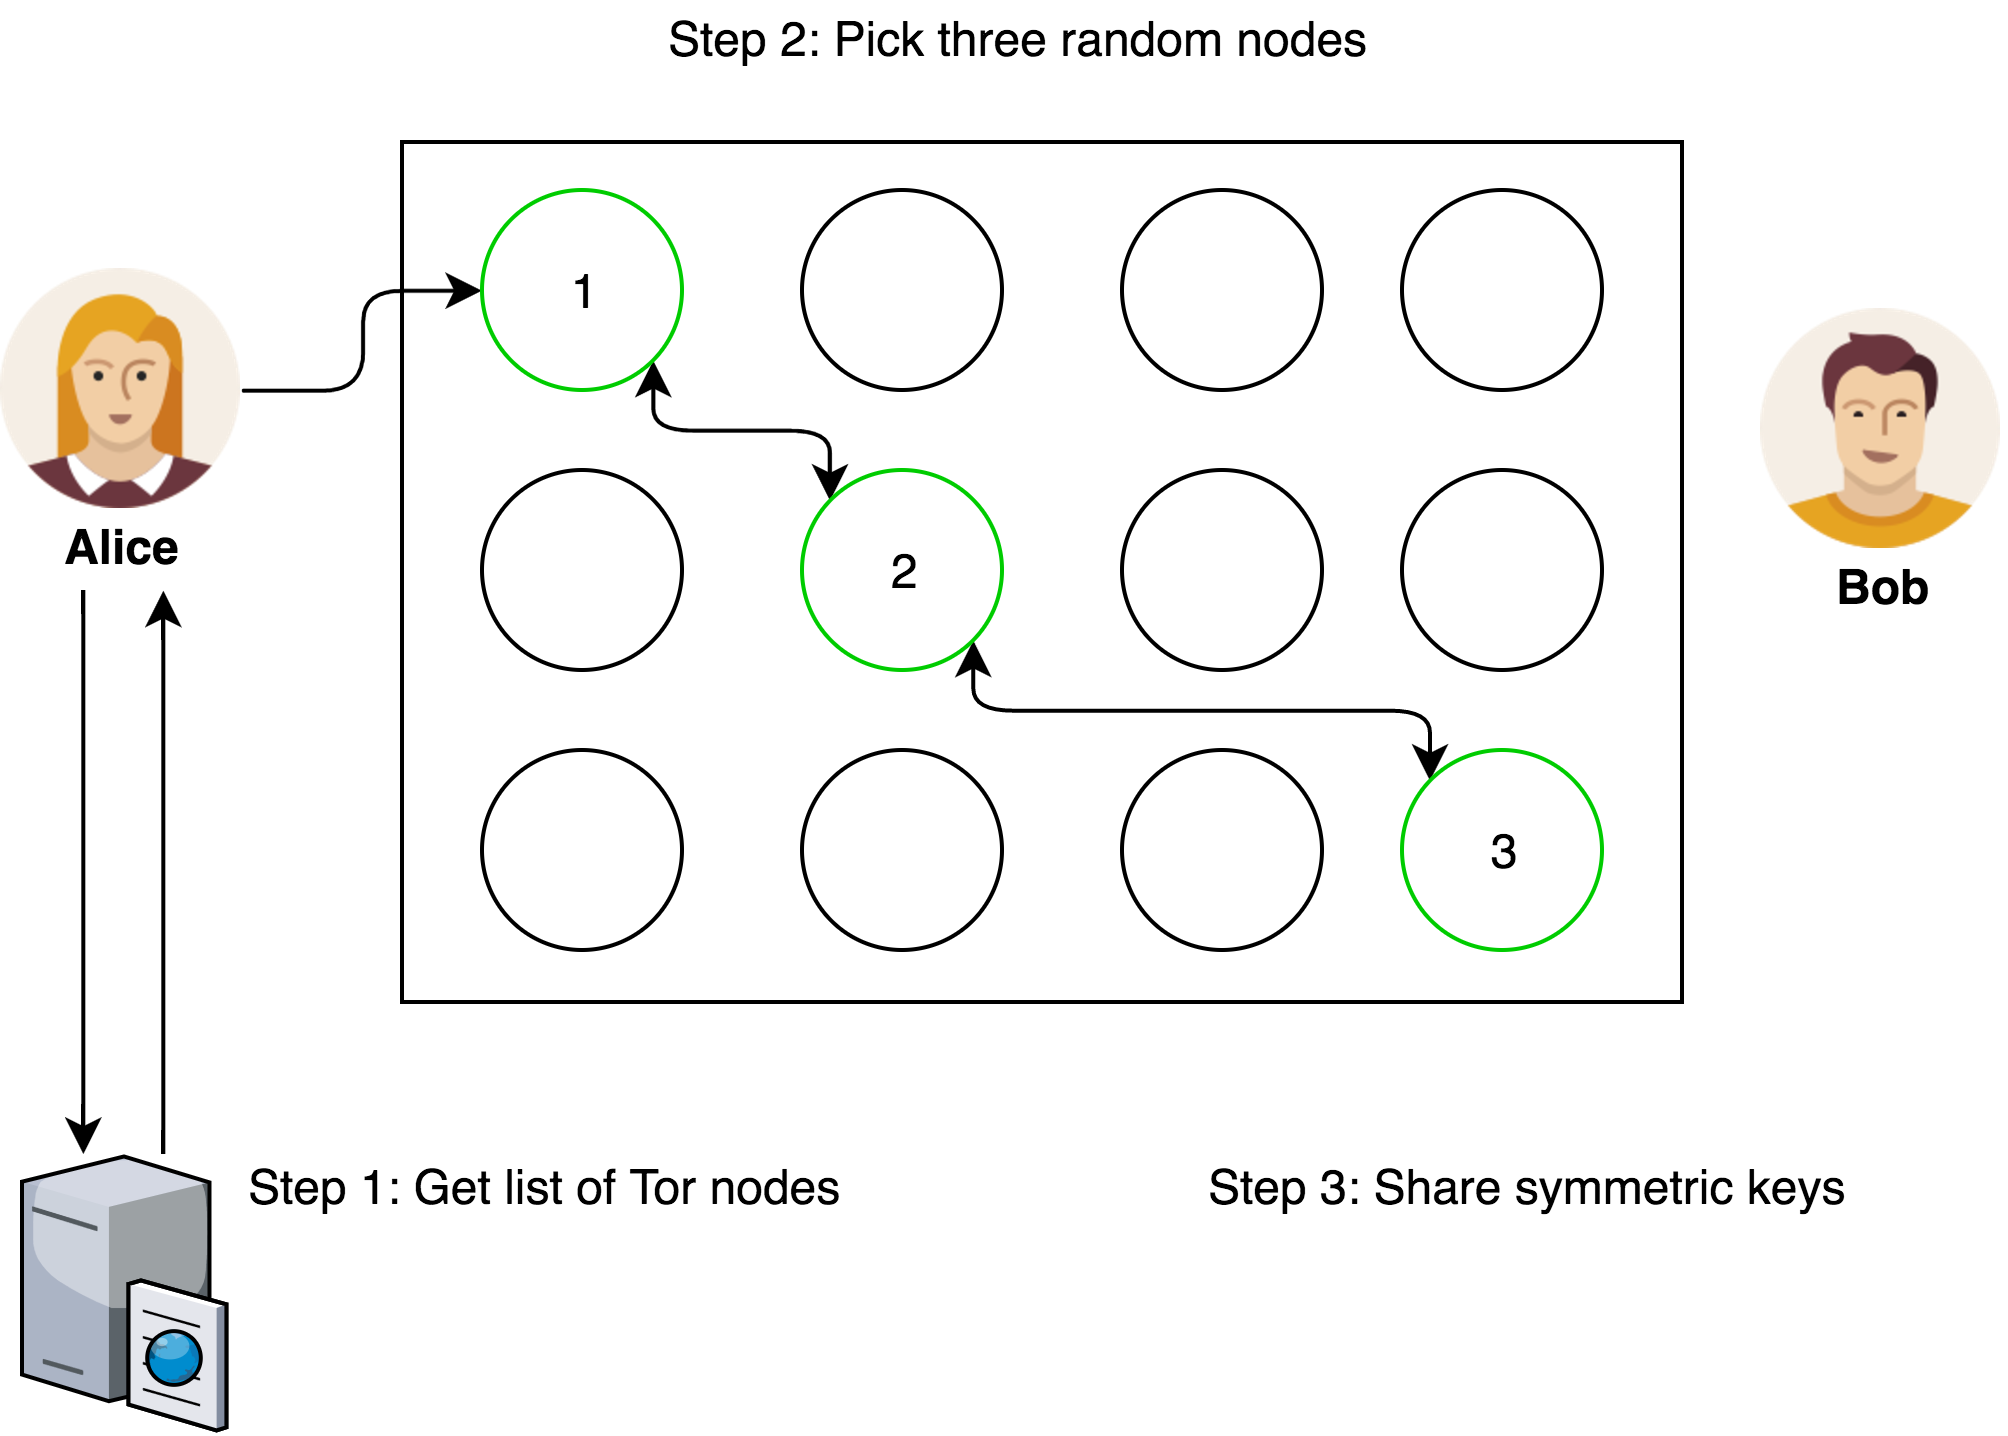
\includegraphics[width=0.75\textwidth]{tor_setup}
      \caption{An example of a connection setup for the onion routing protocol.}
      \label{fig:tor_setup}
    \end{figure}

  \item \textbf{Data Movement:}
    \begin{itemize}
      \item Before Alice can send any data, it first needs to encrypt it in different layers. By this we mean that first it encrypts the data \textit{(with Bob's address)}
        using the shared key from the third node. Next, it encrypts that data again \textit{(with the address of the third node)} using the key from the second node.
        Finally, as expected, it encrypts the data a final time \textit{(with the address of the second node)} using the shared key from the first node.

      \item Now Alice is ready to send the data to the first node.
      \item Once the first node received the data, it decrypts it using the shared key. This reveals the address to the second node.
        The key is here that the first node cannot see the data nor where it is going, since that is still encrypted.

      \item Next, the first node forwards the data that it just unencrypted to the second node. Again, this node decrypts the data, revealing the address to the third node
        but now it doesn't know what the data is, where the final destination is or where it originally came from.

      \item Lastly, the second node forwards the data to the third node. After encryption, this final node can see the data and where it is going but it does not know where it came from.
        So it forwards the data to Bob and not a single party should be able to know the data, the final destination and where it originally came from except for Alice and Bob.
    \end{itemize}

    Now we know why the protocol is called onion routing because it encrypts the data in multiple layers and at every node, one of the layers of the onion is peeled off \cite{tor_project2}.
    The key is that none of the nodes know the complete path that has been taken.

    \begin{figure}[h]
      \centering
      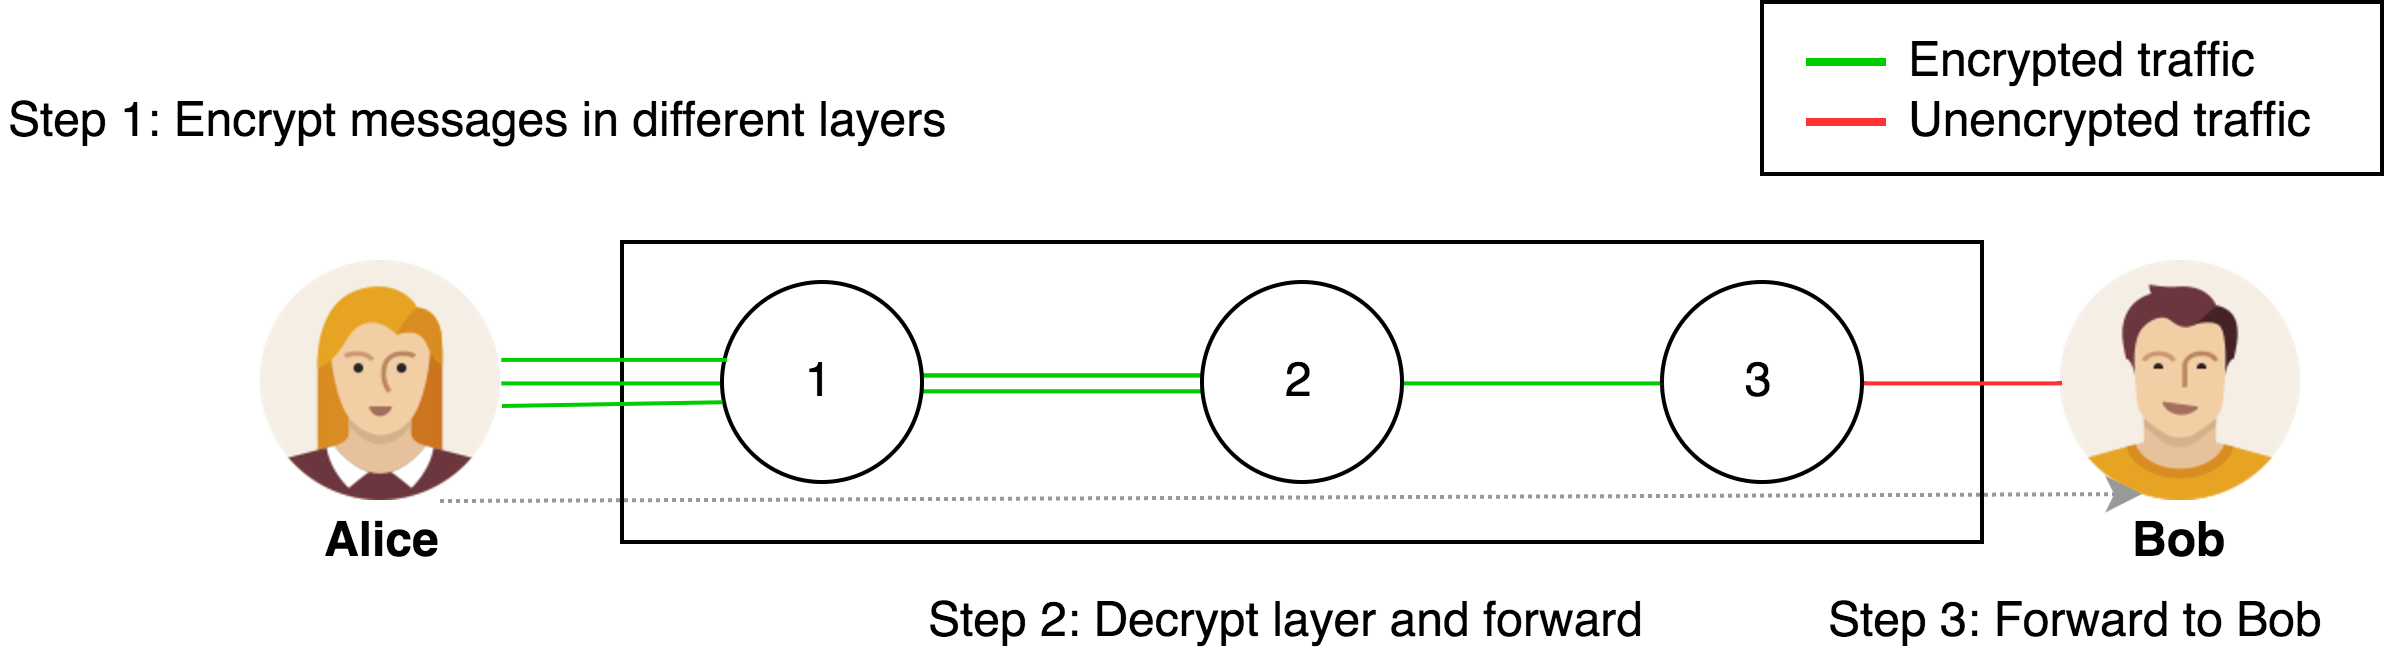
\includegraphics[width=0.75\textwidth]{tor_message_sending}
      \caption{Sending a message with the onion routing protocol.}
      \label{fig:tor_message_sending}
    \end{figure}

  \item \textbf{Connection Tear-down:} This can be initiated by any of the nodes or the client and the process is very straightforward.
    Either the client sends a request for a tear-down to the first node to remove any data on the connection (including the shared key), which is then forwarded to the other nodes.
    Or one of the nodes sends a tear-down message to both the previous node and the next node, which are then forwarded in both directions \cite{goldschlag1999onion}.

\end{enumerate}

Tor generally uses the same circuit for connections that happen within around 10 minutes after creating a circuit.
Later requests, however, are given a new circuit \cite{tor_project, tor_project2}.

\subsection{Related Work}

\subsubsection{Website Fingerprinting}

Website fingerprinting (WF) is the process of attempting to identify which web pages a specific client visits by analysing their traffic traces.
Hence, an attacker is considered to be \textit{local} . By this we mean that they can eavesdrop on the traffic between the client and the first Tor node, as shown in figure \ref{fig:threat_model}.
So it can be anyone from a person on the same network to an ISP.
The reason as to why the attacker has to be local is because in onion routing systems, it is the only place in the network where you still know
the true identity of the client.

\begin{figure}[h]
  \centering
  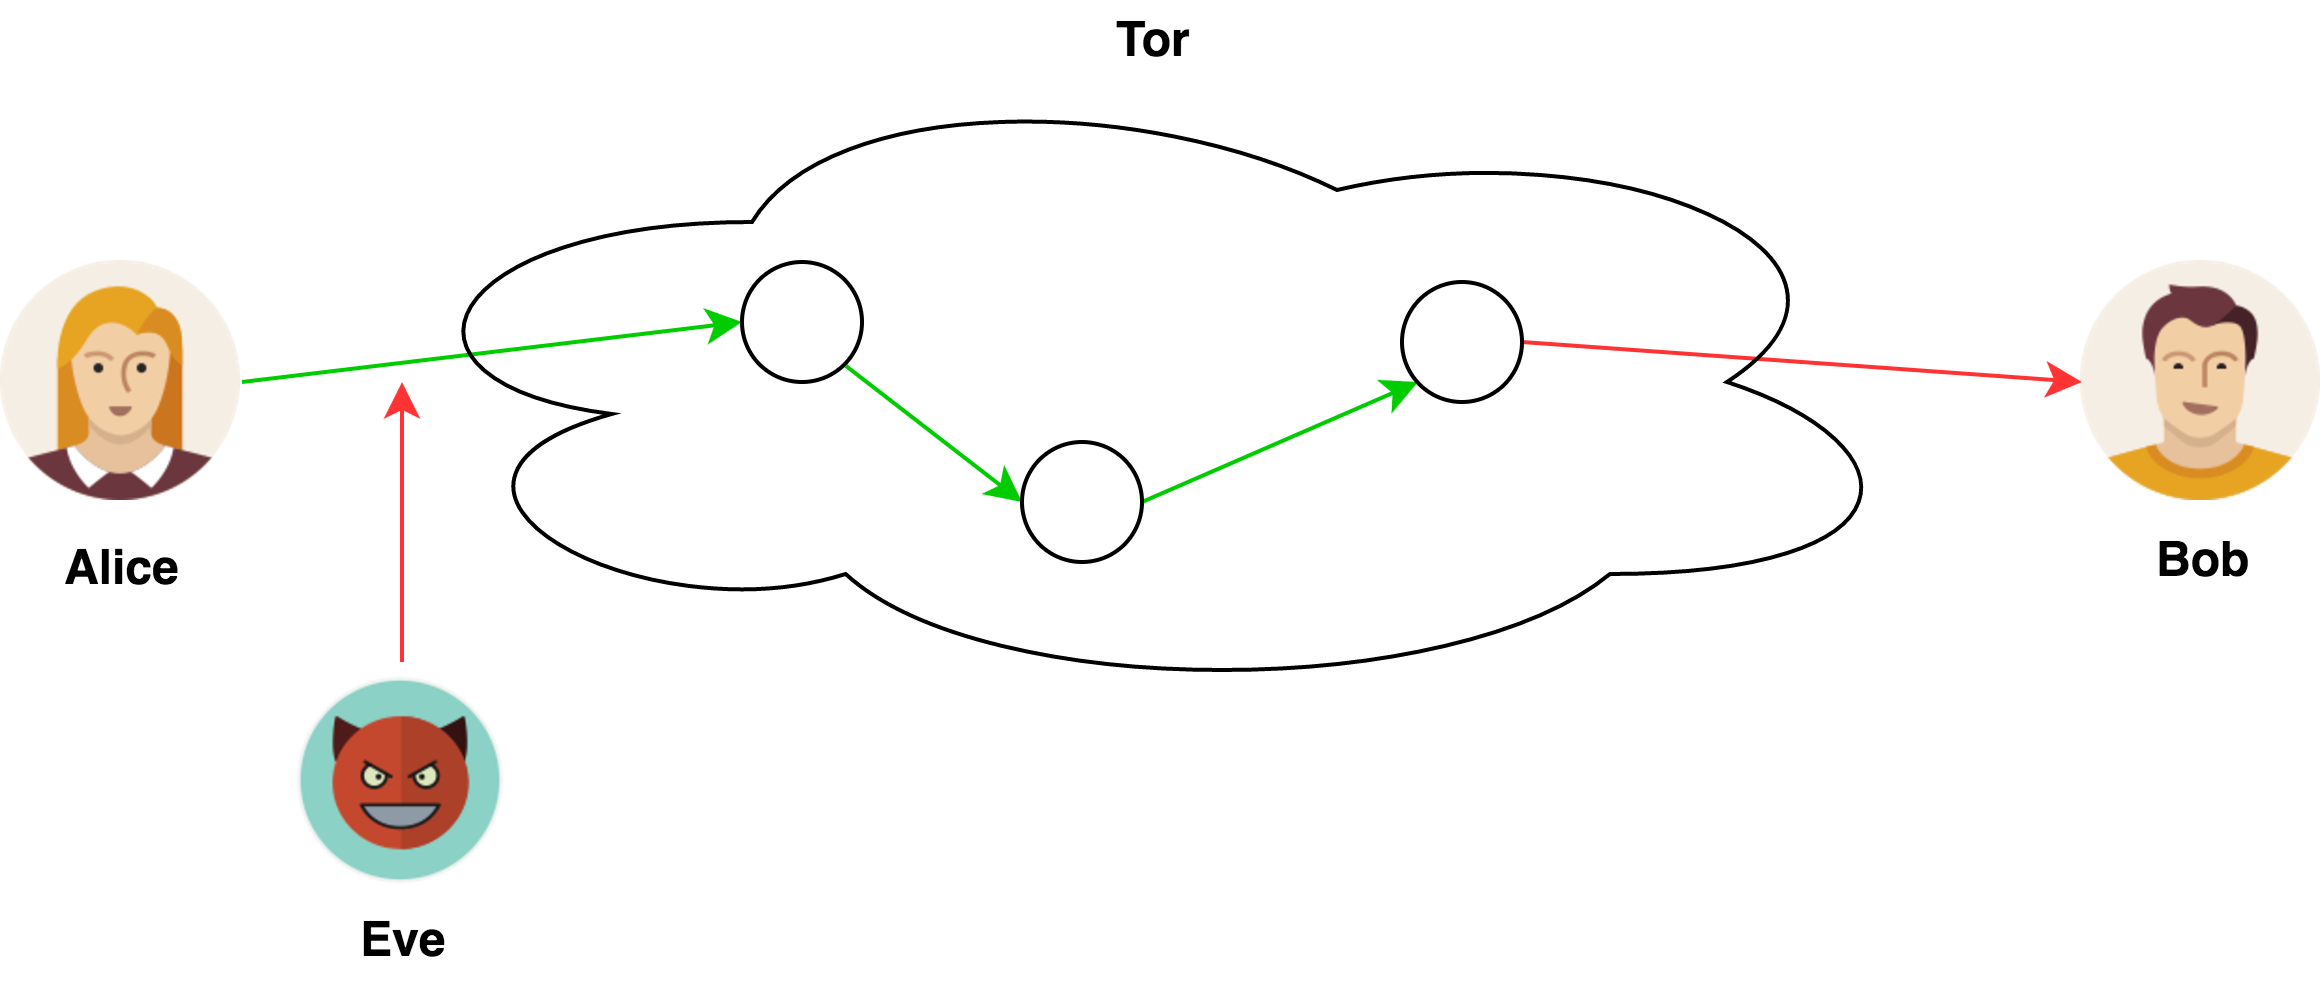
\includegraphics[width=0.75\textwidth]{threat_model}
  \caption{Threat model for a simple website fingerprinting attack.}
  \label{fig:threat_model}
\end{figure}

In general, the attack is as follows. The attacker first collects a dataset that contains packet traces for loading several web pages.
In practice, these web pages are the ones that an attacker is interested in monitoring.
From those traces, the attacker extracts a fixed number of features, the so-called \textit{fingerprint}.
Next, it uses those fingerprints to train some sort of model \textit{(often a machine learning model)} to find patterns in the data.
The attacker observes packet traces, generated by the client, and uses the model to classify which web pages the user is visiting.
Therefore, an attack is essentially a classification problem, where you try to map packet traces into web pages.

We should denote that throughout this report, we will be using the word ``web pages'' rather than ``websites''.
The reasoning behind this is that a website often consists of multiple HTML documents,
which can result in significantly different traffic traces, depending on which document you load.

The term \textit{``website fingerprinting''} was first mentioned by A. Hintz who performed a simple traffic analysis on Safeweb,
an encrypting web proxy that tried to protect user's privacy \cite{hintz2002fingerprinting}. Although the attack was very simple, it and other earlier
works show the possibility that encrypted channels might still leak information about the URL \cite{hintz2002fingerprinting, wagner1996analysis}.
Later, in 2009, the first fingerprinting attack against Tor was executed by Herrmann et al. using a \textit{Multinomial Naive Bayes} model.
They managed to get a relatively high accuracy for several protocols, such as \textit{OpenSSL} and \textit{OpenVPN}, on a small set of 775 web pages.
However on more specialised anonymization networks, the model only achieved a 2.96\% for Tor, which they said was caused by a suboptimal configuration \cite{herrmann2009website}.

Around the same period Y. Shi et al. performed an attack that specifically focused on anonymity systems such as Tor \cite{shi2009fingerprinting}.
Using a cosine similarity, they achieved around 50\% accuracy on an even smaller dataset of only 20 web pages \cite{shi2009fingerprinting}.
The first real threat however, was by A. Panchenko et al. who used a \textit{Support Vector Classifier} (SVC) on the same dataset of 775 web pages as Herrmann et al.
and got a 54.61\% success rate \cite{herrmann2009website, panchenko1}.

All of the previously mentioned research, except the one done by Panchenko et al. have only considered a \textit{closed-world scenario}.
A closed-world setting means that all of the web pages are known in advance \cite{panchenko1}.
For instance, when Herrmann et al. trained their model on a dataset of 775 web pages, they made the assumption that a client could only visit one of
those web pages and none other.
In an \textit{open-world scenario}, the attacker does not know in advance which URLs the victim might visit.
The most prominent example of this is when the authorities want to monitor which people try to access a set of censored sites \cite{panchenko1}.
In order to achieve this, the models need to be trained on both \textit{monitored} and \textit{unmonited web pages}.

Wang et al. later conducted an attack on Tor using a large open-world dataset \cite{wang_cai_johnson_nithyanand_goldberg_2014}.
Using a novel \textit{k-Nearest Neighbor} (k-NN) classifier with \textit{weight adjustment} on a very large feature set \textit{(3736 features)}.
In addition to getting around 90\% accuracy, they also significantly reduced the time needed for training \cite{wang_cai_johnson_nithyanand_goldberg_2014}.

Using a completely different approach, Hayes et al. extract fingerprints using a \textit{random forests} \cite{kfingerprinting}.
This novel technique involved storing a \textit{fingerprint} as a set of leaves within that forest.
Next, they simply use the \textit{hamming distance} as a distance metric to find the k-nearest neighbors.
If all the labels within those $k$ instances are the same, the model classifies the new instance as the previously mentioned label.
The interesting aspect is that changing the value of $k$ allows them to vary the number of \textit{true positives} (TP) and \textit{false positives} (FP) \cite{kfingerprinting}.

Finally, Panchenko et al. improved upon their previous attack to create one current state-of-the-art methods. They tested their approach on several datasets,
including the one used by Wang et al. on their k-NN attack, where they got around 92\% accuracy.
In an open-world scenario, on the other hand, they got up to 96\% accuracy.

\subsubsection{Defenses}

Not only has there been research regarding different attacks but there are also various works that describe possible defenses.
First of all, Tor already implements \textit{padding}, which means that all packets are padded to a fixed-sized cell of $512$ bytes.
Next, in response to the first attack by Panchenko et al., Tor also supported randomized ordering of HTTP pipelines \cite{panchenko1, kfingerprinting, perry2011experimental}.
Finally, on top of these defenses, fingerprinting on Tor is made more difficult by all of the background noise present.
This is due to the fact that Tor also sends packets for circuit construction or just \textit{SENDME's}, which ensure flow control \cite{panchenko2}.
Although Wang et al. proposed a probabilistic method to remove these \cite{wang_goldberg_2013}, they might still make the classification process slightly more difficult.

Lua et al. designed an application-level defense, that was able to successfully defends against a number of classifiers by modifying packet size, timing of packets, web object size, and
flow size \cite{perry2011experimental}. This is achieved by splitting individual HTTP requests into multiple partial requests, using extra HTTP traffic as a cover and making use of HTTP pipelining \cite{cai_zhang_joshi_johnson_2012}.
Although this has been a relatively effective technique to obfuscate traffic, several attacks have proven that this defense only still does not suffice \cite{cai_zhang_joshi_johnson_2012,wang_cai_johnson_nithyanand_goldberg_2014}.

\textit{BuFLO}, on the other hand, is a \textit{simulatable} defense \cite{wang_cai_johnson_nithyanand_goldberg_2014}, designed by Dyer et al. that performed packet padding and sending data at a constant rate in both directions \cite{dyer2012peek}.
The disadvantage of this method is the high overhead required in order to keep the constant data rate.
Some extensions have been described that try to minimize this overhead such as  Nithyanand's work that uses existing knowledge of a website traces to maintain a high level of security \cite{nithyanand2014glove}.

More recently, Cherubin et al. developed the first website fingerprinting defense on the server side \cite{cherubin2017website}.
This can be particularly interesting for \textit{Tor hidden services} that want to provide, all of their users, the privacy that they require.
The attack uses a technique, called \textit{ALPaCA}, which pads the content of a web page and creates new content to conceal specific features on a network level \cite{cherubin2017website}.

Finally, there are also some other techniques such as \textit{decoy pages} and \textit{traffic morphing} \cite{wright2009traffic,panchenko1}.
Decoy pages or \textit{camouflage} is a very simple technique that involves loading another web page whenever a web page is requested.
This process provides more background noise that makes fingerprinting more difficult \cite{panchenko1}.
Whilst traffic morphing is a slightly more complex technique that changes certain features in the traffic in order to make it appear as if another page is loaded \cite{wright2009traffic}.

\subsubsection{Critical Analysis}
- Examine how would a small percentage of false positives impacts a potential attack.
- Analyse how the rapid changing nature of some web pages would impact the attack.
- Tor version
- Closed world
- Well defined packet traces (It is assumed that the attacker knows where the packet trace of a single page load starts and ends. If the client takes much
    longer to load the next page after the current one is loaded, this assumption can be justified.)
- No other activity (multi-tab browsing)
- Dynamic websites
- Adversary (ISP) can block Tor

(Website fingerprinting at Internet scale proves that the attack does not scale in realistic settings)

\subsection{Deep Learning}

\subsection{Automatic Feature Selection}

\subsubsection{Stacked Authoencoder}

\subsubsection{Sequence-to-Sequence Model}

\subsection{Software Libraries}

  \chapter{Attack Design}

In this section, we describe the overall design of our automatic feature generation models, outline the attack strategy and explain certain design decisions.
Most of this section will be split into two different parts.
First, we describe the feature generation processes and then the overall attack.

\section{Stacked Autoencoder}

A stacked autoencoder takes a fixed-length input vector and tries to learn a function that compresses that vector.
Thus if we were to use it for a fingerprinting extraction task, we will need to preprocess the variable-length traces into a fixed-length input.
There are various different manners of doing this.
One of the most naive ones is to find the longest length trace and pad all of the other traces up to that length.
However, in Greschbach et al.'s dataset, this length is around $250,000$ \cite{greschbach2016effect}, which means that our network will need to be incredibly deep to extract a short trace.

Instead, we can pick the average or median length of the traces and cut or pad traces which are longer or shorter.
In this work we will investigate the average length, which is around $3,000$.
But the median length might be slightly more appropriate, as the length is positively skewed.
On top of that, we deal with the fact that each packet is represented by a tuple, by just multiplying the time by the direction.
Therefore, all of the outgoing packets are positive whilst the incoming ones will be negative.

Finally, since the output of the activation functions used is either between 0 and 1 or -1 and 1, we will scale the inputs accordingly.

\section{Sequence-to-Sequence Model}

As described in section \ref{sec:seq2seq}, a sequence-to-sequence model is able to learn how to construct a fixed-length representation from a variable-length sequence, which means that we will not have to perform as much preprocessing as for our autoencoder.

Although we already know the overall structure, there are still a couple of design decisions that had to be made specifically for our attack.
These decisions are outlined in the following section.

One of the first parameters which we will examine is the \textit{amount of hidden states} in the RNN cells.
This number affects the amount of neurons for each layer with the cells.
For instance if the amount of hidden states is set to $100$, the state of an LSTM cell is represented by vector of length $200$ (two vectors of length $100$).
The higher this number, the easier it should be to learn a representation, as the compression factor is lower.
But we also need to consider the fact that the higher the amount of hidden neurons, the more variables the model needs to learn and thus the more complex the model will be are.

Each value in a trace can be represented by a vector of length two (timestamp and direction), as seen in table \ref{table:cell-extract}.
Therefore, if the amount of hidden cells is not equal to two, we will also need to \textit{project} the input and output vectors into the necessary dimensions.

\begin{figure}[ht]
  \centering
  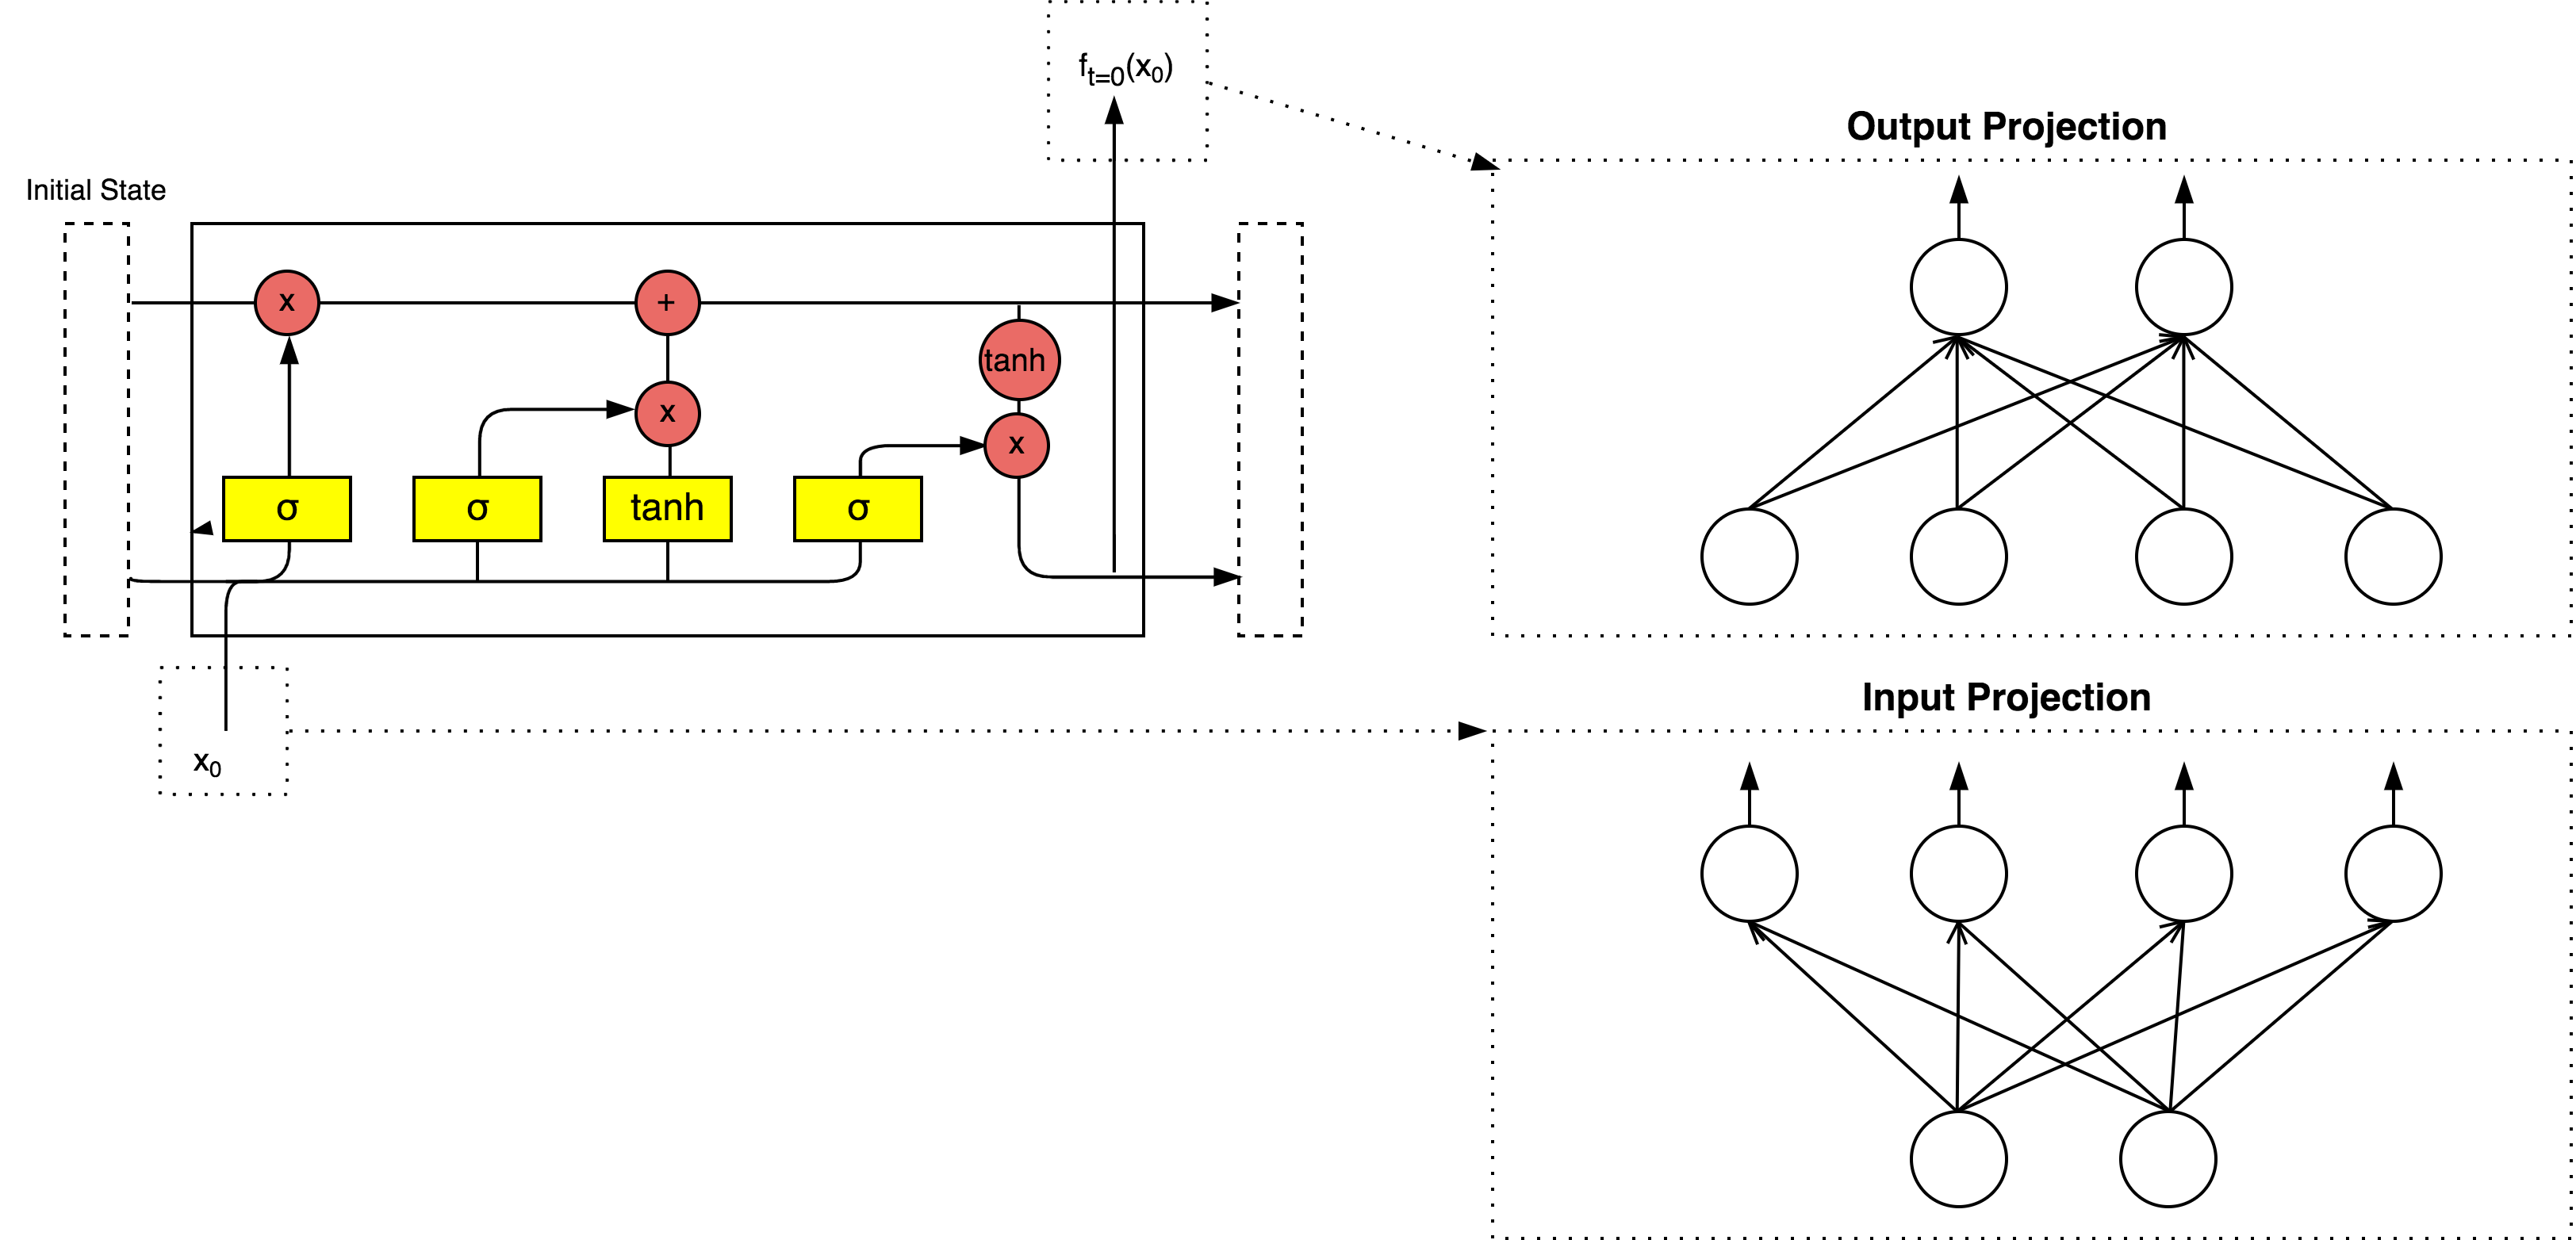
\includegraphics[width=0.7\textwidth]{lstm-projection}
  \caption{Example of projection within a LSTM cell with 4 hidden states.}
  \label{fig:lstm-projection}
\end{figure}

\newpage

Some of the traces can be particularly long and therefore the network needs to be unrolled to extreme lengths \cite{greschbach2016effect}.
In fact, given memory constraints, this becomes a major problem.
But it can be solved by cutting the traces after a couple seconds since it has been shown that the first part of a trace carries more information than the latter.

\begin{figure}[ht]
  \centering
  
\includegraphics[width=\textwidth]{full-seq2seq}
  \caption{Overal structure of our sequence-to-sequence model.}
  \label{fig:full-seq2seq}
\end{figure}

Based on the above, we can construct our \textit{computational graph} in Tensorflow as outlined in figure \ref{fig:full-seq2seq}.

\section{Attack Strategy}

Here we consider an adversary that relies on deep learning to extract fingerprints for a website fingerprinting attack.
This adversary can have two different goals in mind, as previously stated in section \ref{sec:threat-model}.
The full attack, however, can be split up into four different stages, namely \textit{data collection}, \textit{fingerprint extraction training}, \textit{classifier training} and \textit{the attack}.

\noindent
\textbf{Data Collection}
\begin{enumerate}
  \item Choose web pages that the attacker wishes to monitor.
  \item Collect traffic for a set of monitored and unmonitored sites.
  \item Convert the raw TCP data into Tor cells.
  \item Remove SENDMEs and other noise.
\end{enumerate}

\noindent
\textbf{Fingerprint Extraction Training}
\begin{enumerate}[resume]
  \item Further process the data into batches and perform any other preprocessing required by the model such as cutting or padding the traces.
  \item Prepare the fingerprint extraction model.
  \item Train the fingerprint extraction model on a copy task for monitored and some unmonitored web pages.
  \item Extract fingerprints from data by using the trained model.
\end{enumerate}

\noindent
\textbf{Classifier Training}
\begin{enumerate}[resume]
  \item Given a classifier, train it using the extracted fingerprints.
  \item Measure performance of classifier.
\end{enumerate}

\noindent
\textbf{The Attack}
\begin{enumerate}[resume]
  \item Passively capture traffic from Tor users.
  \item Pre-process the collected data.
  \item Extract fingerprints using the trained fingerprint extraction model.
  \item Classification via the trained classifier.
\end{enumerate}

\begin{figure}[ht]
  \centering
  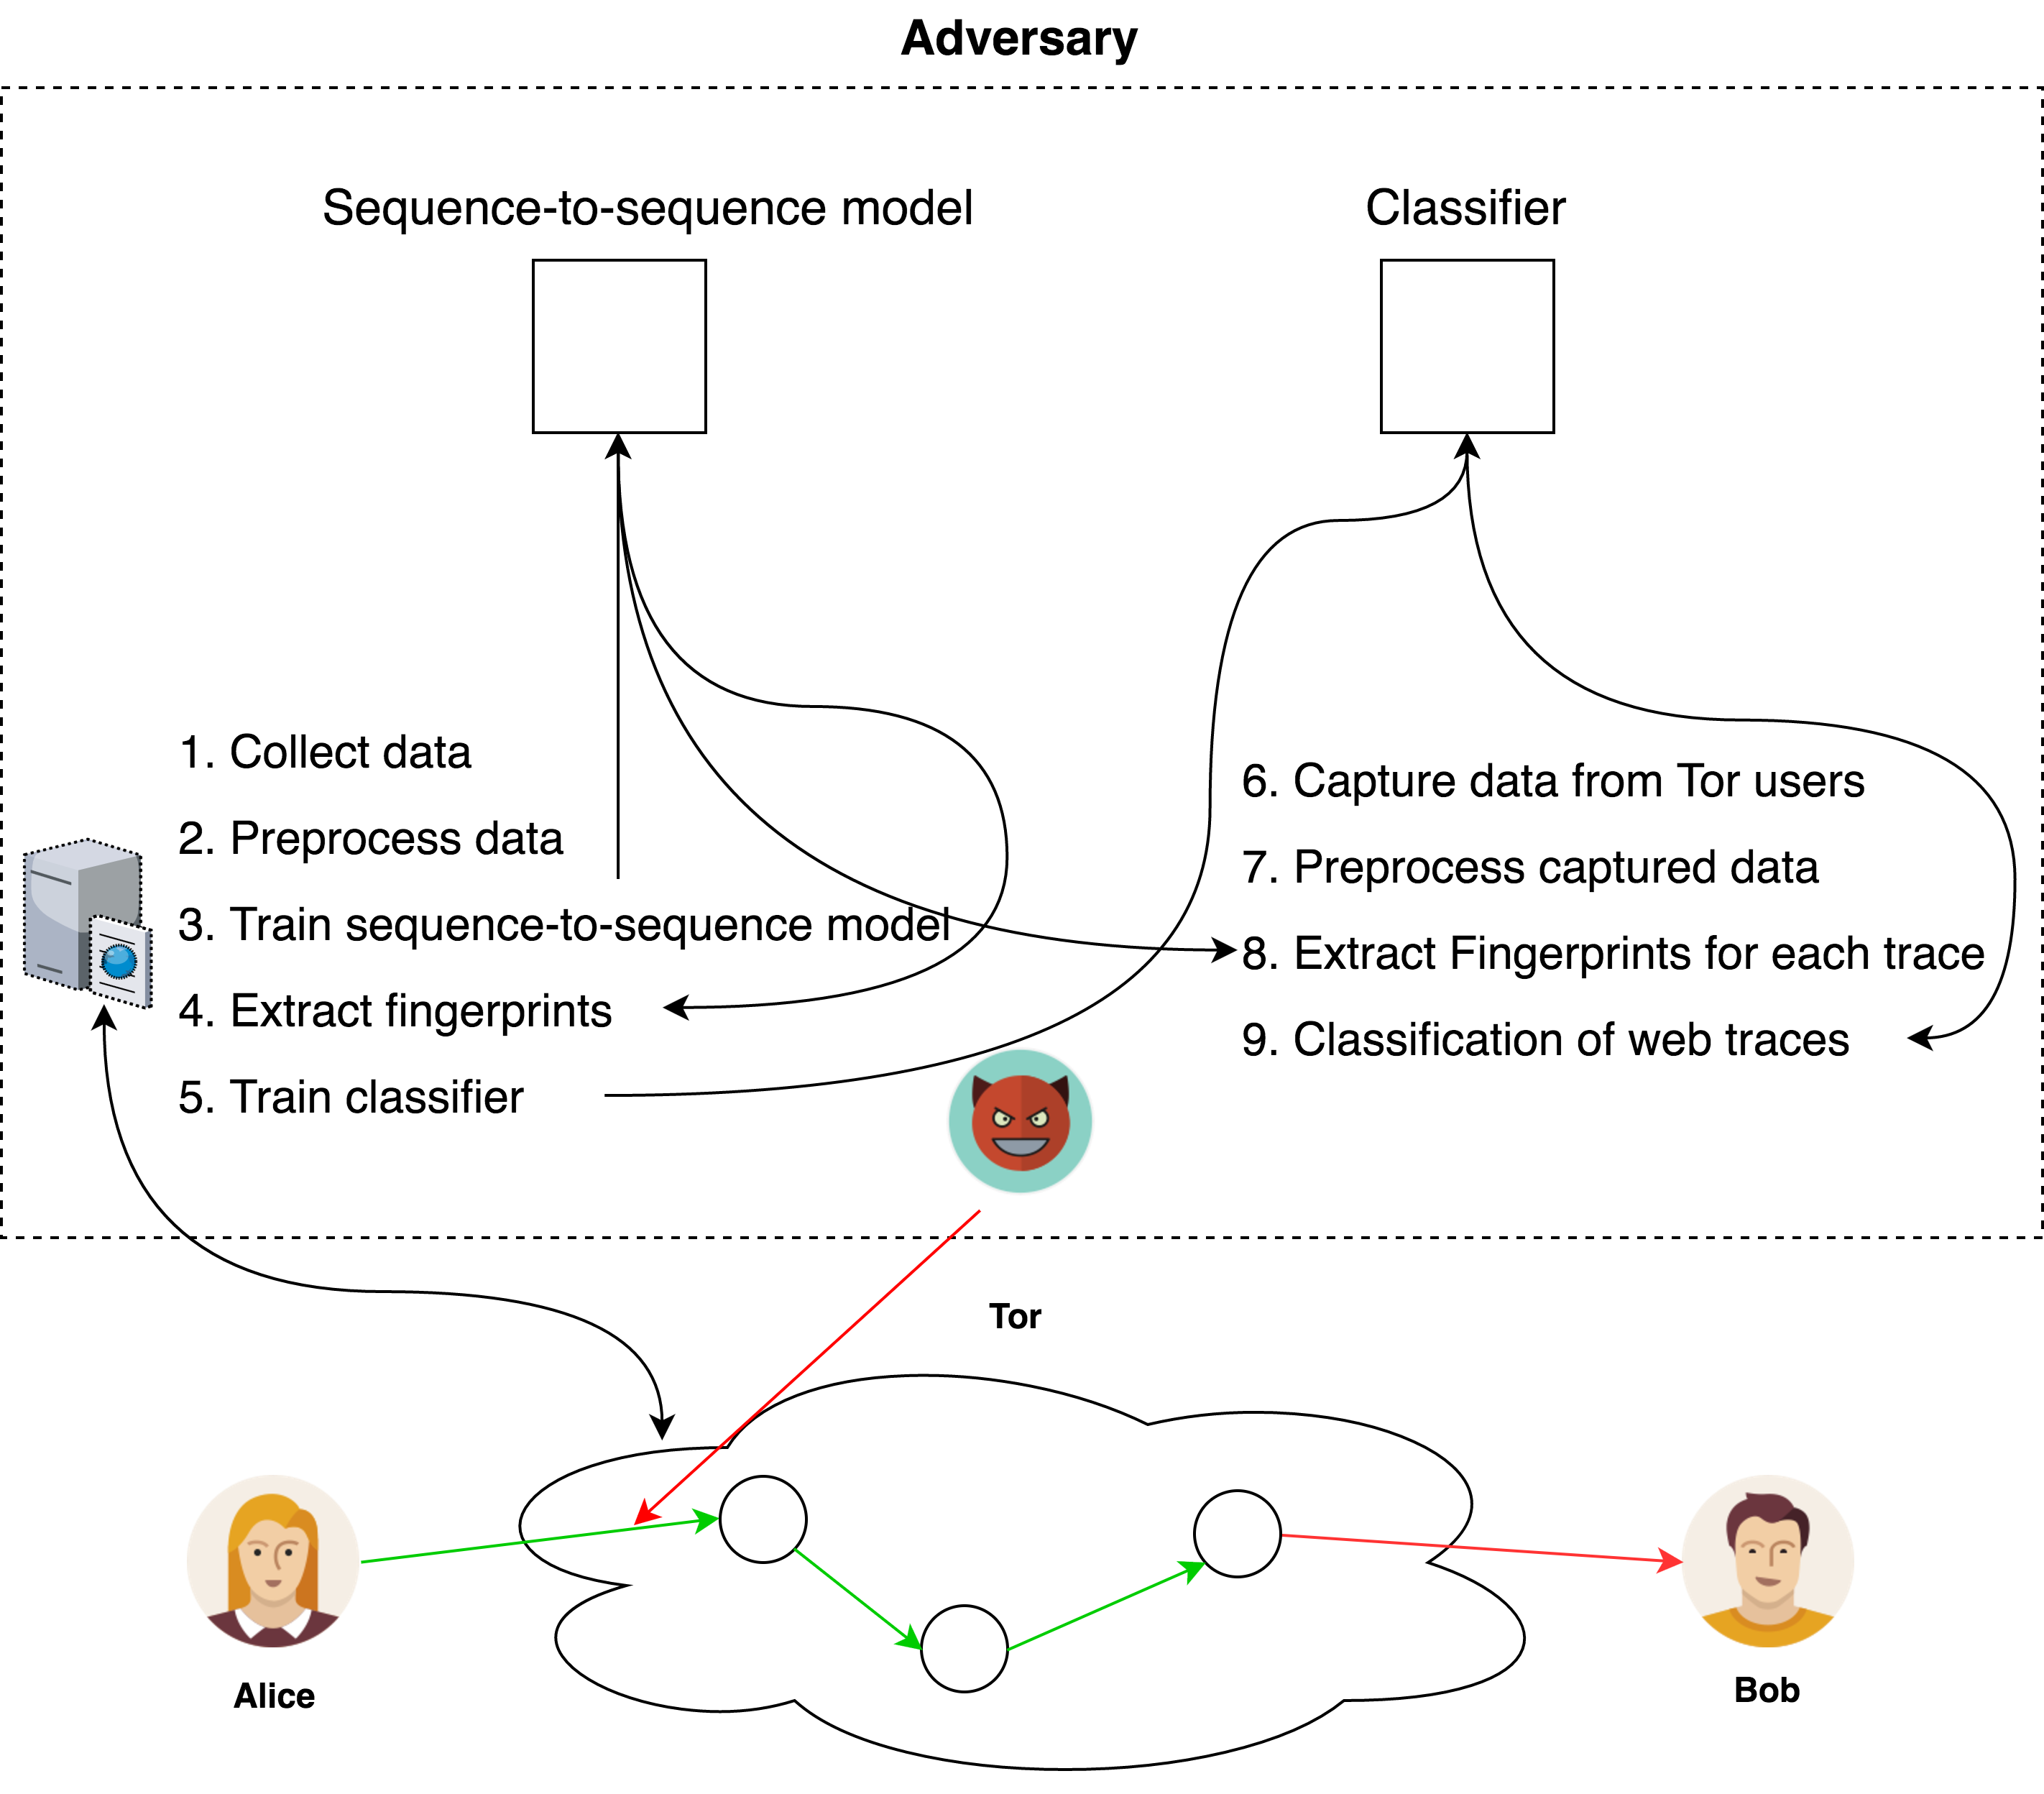
\includegraphics[width=0.7\textwidth]{overall-structure}
  \caption{Attack strategy.}
  \label{fig:attack-strategy}
\end{figure}

\subsection{Data Collection} \label{sec:data_collection1}

As previously mentioned, the data collection process first requires the adversary to choose a set of $n$ websites to monitor.
Next, the adversary crawls these pages a total of $i$ iterations to ensure that a classifier has enough data to generalize.
As suggested by Wang et al. when performing page loads, browser caching should be disabled since Tor does not allow caching to disk and therefore the browser cache should be cleared every time a web page is loaded \cite{wang_goldberg_2013}.
After the collection, the TCP data is converted into Tor cells and probabilistic algorithms, designed by Wang et al. \cite{wang_goldberg_2013}, are used to remove SENDMEs from the data.
This data can be processed further, however we chose not to since the model should be able to learn how to perform this processing.

Most of our analysis will be done using the dataset provided by Greschbach et al. \cite{greschbach2016effect}, which can be used for open-world analysis since it provides us with $100$ samples for Alexa's top $9000$ websites and one sample of one sample for $909,000$ unmonitored sites.
For the rest of this paper, we will refer to this dataset as \texttt{GRESCHBACH}.
Next, to see how our model performs on data, which was recorded at a different time and under different circumstances, we will also be using the dataset provided by Wang et al. \cite{wang_cai_johnson_nithyanand_goldberg_2014}, which we will call \texttt{WANG14} \cite{panchenko2}.
This set is slightly smaller with $100$ monitored websites with $90$ instances each and $8400$ unmonitored sites.

\subsection{Fingerprint Extraction Training} \label{sec:fingerprint-extraction-training}

In order to truly evaluate the model, we need to split the data up into a training and a validation set.
We do not train the model on any data in the validation set but instead use it to see how well the model performs on unseen data.
For this split, we use a \textit{stratified shuffle split}, meaning that we shuffle the data and then perform the split, whilst preserving the class distributions.
On top of training the feature extractor with monitored pages, we also train it on unmonitored pages, as it needs to be able to extract features effectively from both sets.

During training and extracting the fingerprints, \textit{mini-batch processing} will always be used.
This will allow us to gain a performance boost and perhaps even have a faster convergence.
When dividing the data up into these batches, we also need to determine how big they will be.
The bigger they are, the larger the performance gain will be but the lower the accuracy might be.
Additionally, the size of the batches also depend on the amount of available memory since we cannot have the VM run out of memory whilst training.

On top of determining the batch size, the individual models require different preprocessing steps and tuning of different parameters.

\subsubsection{Stacked Autoencoder}

As previously mentioned, after dividing the data up into batches, we either need to cut or pad the traces such that they all are of a fixed-length.
Next, we know that the first layer needs to have the same amount of neurons than the length of the input.
But after that, there are a variety of different architectures that need to be chosen.
Some of which are outlined below:

\newpage

\begin{itemize}
  \item How many hidden layers we want.
    The more there are, the more complex the function that can be modeled but also the harder it becomes to train the model.

  \item The amount of hidden neurons in each layer.
    This number should gradually decrease to the number of features we would like to extract.

  \item The activation function of the neurons.
    The most popular ones being \textit{sigmoid}, \textit{ReLu} and an \textit{atan}.

  \item Whether or not to include batch normalization at every step.
\end{itemize}

After that the model has been constructed, there are still several learning parameters that need to be tuned:

\begin{itemize}
    \item The optimizer to use (\textit{adam}, \textit{gradient descent} or \textit{RMSProp}) \cite{tensorflow}.
    \item Learning rate ($\gamma$) for the previously chosen optimizer.
    \item Amount of traces within a single mini-batch ($m$).
    \item Cost, or loss function ($f$) to minimize (\textit{mean squared error} (MSE), \textit{absolute loss} (AL) or \textit{cross-entropy}) \cite{tensorflow}.
\end{itemize}

\subsubsection{Sequence-to-Sequence Model}

Each batch can either be presented in \textit{batch-major} or \textit{time-major} form.
Although time-major is slightly more efficient \cite{tensorflow}, we opt for a batch-major form, since it makes the fingerprint extraction process easier.
Next, after the data has been divided into mini-batches, we perform some further processing such as cutting the traces after several seconds.
Finally, since all of the traces within a batch need to be of the same length, padding is performed as a final preprocessing step.

After collecting and fully preprocessing the data, the adversary can start to construct the sequence-to-sequence model.
However, in order to do so, there are a variety of different architectures that need to be considered, some of which are outlined below:

\begin{itemize}
  \item Which sort or RNN cells to use. The most popular ones being GRU or LSTM cells.
    We could also potentially investigate the usefulness of multilayered RNN cells but we expect the performance gain to be limited, which is why we do not consider them in our evaluation.

  \item Whether or not to use a bidirectional encoder to ensure that the output at time $t$ is not only affected by past information but also on future information.

  \item The amount of hidden states within a RNN cell, which affects the size of the fingerprints.
\end{itemize}

Now that the model has been constructed, the adversary again has to chose various learning parameters such as:

\newpage

\begin{itemize}
  \item The optimizer to use (\textit{adam}, \textit{gradient descent} or \textit{RMSProp}) \cite{tensorflow}.
  \item Learning rate ($\gamma$) for the previously chosen optimizer.
  \item Amount of traces within a single mini-batch ($m$).
  \item Cost, or loss function ($f$) to minimize (\textit{mean squared error} (MSE), \textit{absolute loss} (AL) or \textit{cross-entropy}) \cite{tensorflow}.
  \item After how much time the traces are cut.
\end{itemize}

After these parameters have been tuned, the computational graph can be constructed in Tensorflow and the model can be trained.
When this training has been completed, fingerprints can finally be extracted for all the traces in the test set.

\subsection{Classifier Training} \label{sec:classifier-training}

When the adversary has extracted the fingerprints for websites within the test set, they need to train a classifier on those fingerprints.
Most works so far rely on some sort of \textit{supervised machine learning} techniques such as \textit{support vector classifiers} (SVC), \textit{k-nearest neighbours} (kNN), \textit{random forests} (RF) or \textit{naive bayes} (NB) \cite{panchenko1,panchenko2,wang_cai_johnson_nithyanand_goldberg_2014,kfingerprinting,naivebayes}.
All of these algorithms rely on different techniques but an explanation of their inner workings is outside the scope of this paper.
Instead, we will consider them as \textit{black box models}.
This means that all we know is that we can apply a \texttt{fit} function to the models, which causes them to learn how to classify the fingerprints and a \texttt{predict} function, which predicts the classes of given inputs.

To measure the performance of our black-box models, we use a similar technique as we did in the previous section.
We split our test set up into two more sets, a \textit{classifier training set} and a \textit{classifier test set}.
But since training a classifier, requires less time, we can use another technique, called \textit{stratified k-fold validation}.
Here we split our original test set up into $k$, mutually exclusive, folds.
Next, one of the folds is chosen to be the classifier test set and all of the other folds form the classifier training set.
This process is repeated for $k$ iterations, where at each iteration, a different fold is chosen to be the test set.
But again, we preserve the class distributions within all of the folds.

\begin{figure}[ht]
  \centering
  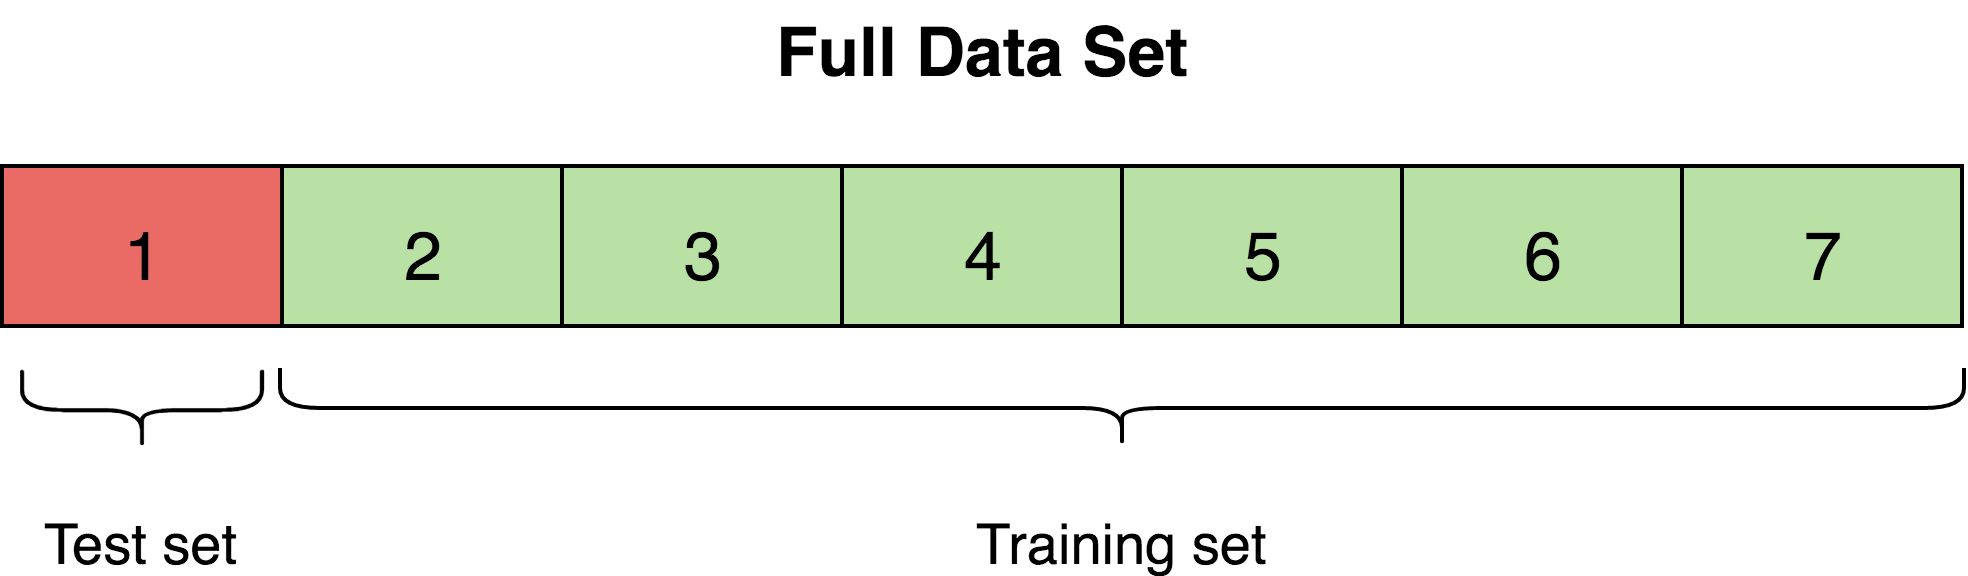
\includegraphics[width=0.6\textwidth]{kfold}
  \caption{Example of one iterations in a k-fold validation $(k = 7)$.}
  \label{fig:kfold}
\end{figure}

For each iteration of the validation process, several statistics can be recorded and then averaged over all iterations.
The k-fold validation process ensures that every data point will be in the test set at least once and therefore giving us an accurate measure of these statistics.

Some of the performance measures that we will use in the evaluation stage are outlined below.
Please note that we describe them within the context of a WF attack:
\begin{itemize}
  \item \textbf{True Positive Rate (TPR)} is the probability that a monitored page is classified as the correct monitored page \cite{kfingerprinting}.

  \item \textbf{False Positive Rate (FPR)} is the probability that an unmonitored page is incorrectly classified as a monitored page \cite{kfingerprinting}

  \item \textbf{Bayesian Detection Rate (BDR)} is the probability that a page corresponds to the correct monitored page, given that the classifier recognized it as that monitored page \cite{kfingerprinting}.
    This can be calculated as follows:
    $$\text{BDR} = \frac{\textit{TPR} \times \Pr(M)}{\textit{TPR} \times \Pr(M) + \textit{FPR} \times \Pr(U)}$$
    where
    $$\Pr(M) = \frac{|\text{Monitored}|}{|\text{Total Pages}|}, \quad \Pr(U) = 1 - \Pr(M)$$

    This measure essentially indicates the practical feasibility of the attack, as the adversary is mainly concerned with this specific measure \cite{kfingerprinting}.

  \item \textbf{Accuracy (A)} is the percentage of correctly classified instances.
    Although it can be used as a rough indicator, it will not be used in the final conclusions because of the \textit{accuracy paradox}, which arises due to class imbalance.

  \item \textbf{F1-Score (F1)} measures the harmonic mean between precision and recall \cite{scikitlearn}.
    \begin{align*}
      \text{F1} &= 2 \times \frac{\text{precision} \times \text{recall}}{\text{precision} + \text{recall}}\\
                &= \frac{2 \times \textit{TP}}{2 \times \textit{TP} + \textit{FP} + \textit{FN}}
    \end{align*}
    where
    $$\text{recall} = \frac{\textit{TP}}{\textit{TP} + \textit{FN}}, \quad \text{precision} = \frac{\textit{TP}}{\textit{TP} + \textit{FP}}$$

    This measure is particularly useful since it is not affected by class imbalance.
\end{itemize}

Rather than using another classifier, we could potentially add a \textit{softmax layer} on top of our encoder, like V. Rimmer uses on top of her stacked autoencoder \cite{deeplearningthesis}.
We could use this idea for both our autoencoder and the sequence-to-sequence model.

This process would involve first training the sequence-to-sequence model, then stacking the softmax layer on top of each unrolled cell in the encoder and using it for classification.
What would be interesting about this approach is that the adversary can analyse how certain the classifier is, as it analyses packets more and more packets from the trace.
But unfortunately this is outside the scope of this paper, as we are solely focusing on the feature extraction process.

\begin{figure}[ht]
  \centering
  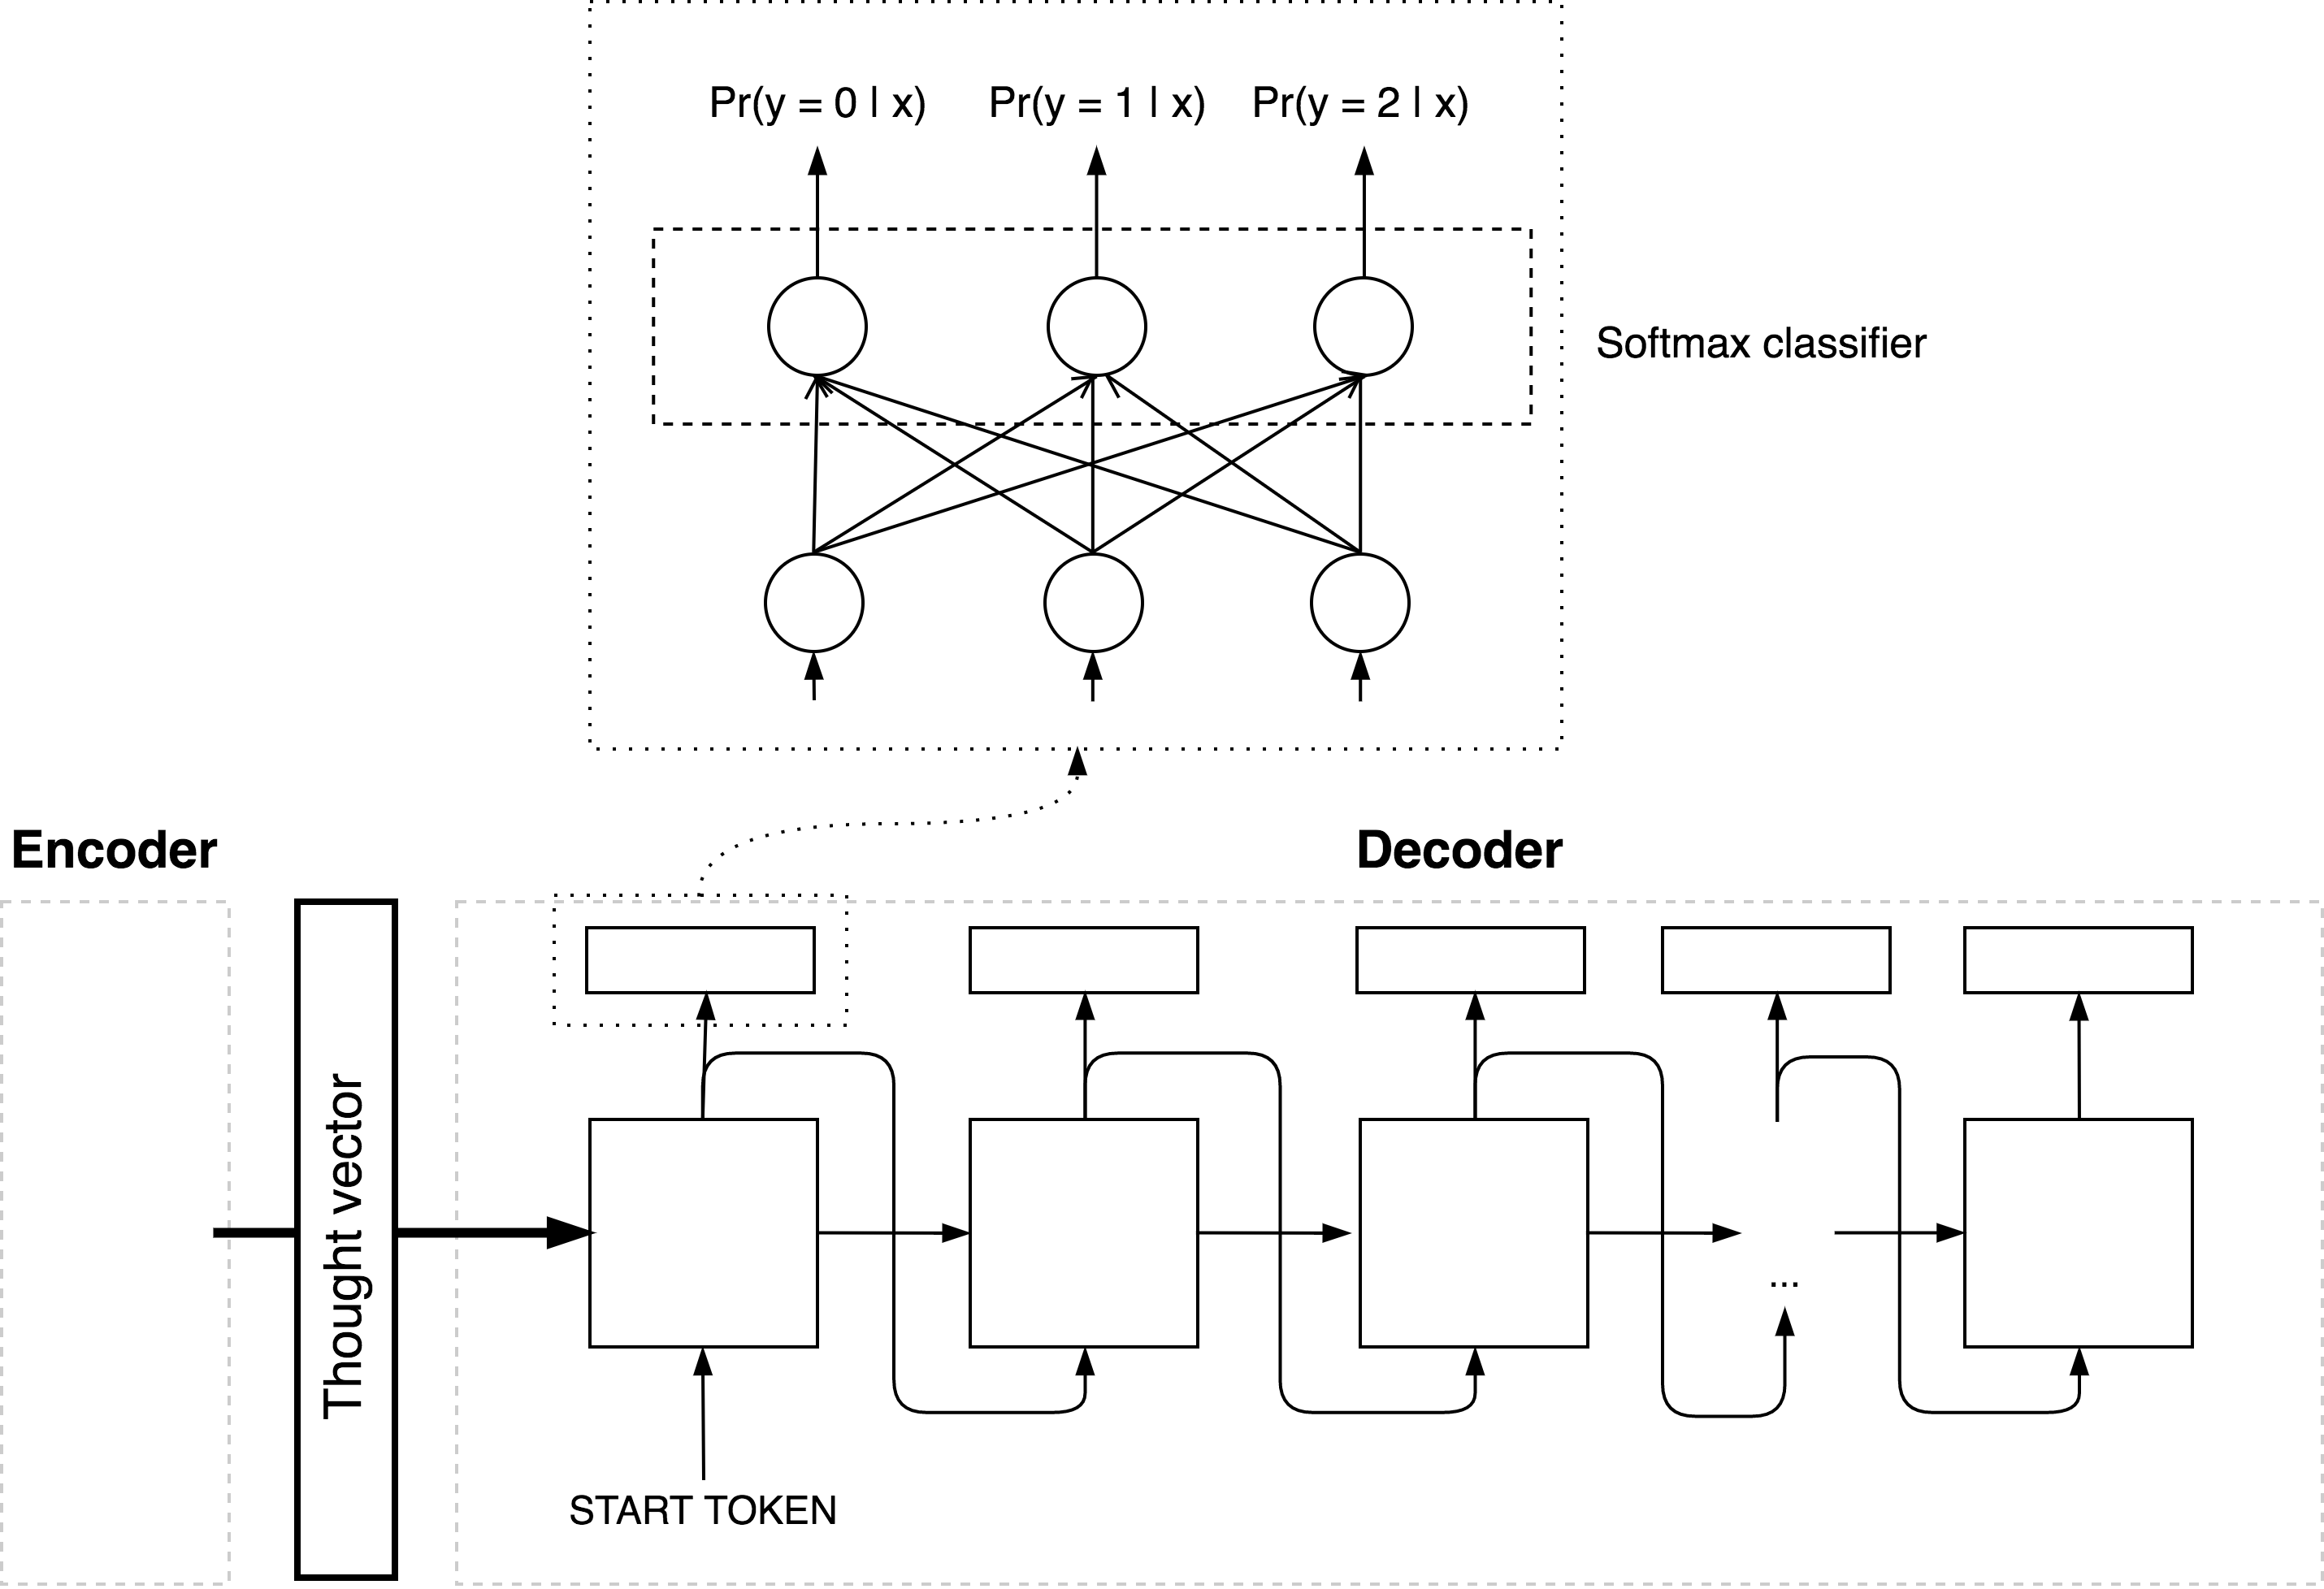
\includegraphics[width=0.55\textwidth]{softmax}
  \caption{Example of encoder with softmax layer for 3 web pages.}
  \label{fig:softmax}
\end{figure}

\newpage

\subsection{The Attack}

Finally, after the adversary has trained the required models, the real WF attack can start.
First, the adversary starts capturing web traffic data between the user and the entry guard, as shown in figure \ref{fig:threat_model}.
Next, the data is preprocessed for the fingerprint extraction process, as described in section \ref{sec:fingerprint-extraction-training}.
After all the preprocessing has finished, fingerprints are extracted using the previously trained model.
Finally, those fingerprints are used as features for a classifier, which classifies the traffic into web pages.

The time between data collection for training and performing the WF has to be kept as small as possible since Juarez et al.'s experiments show that web pages' content changes greatly over time, therefore affecting the accuracy of the attack \cite{wfpevaluation}.

\section{Code Structure} \label{sec:code-structure}

In this work, we will not be conducting the final stage of a WF attack.
Instead, we will be reporting the results on the test sets.
All of this is reflected in the overall structure of the code, which consists of four main components, as can be seen in figure \ref{fig:code-structure}.

\begin{figure}[ht]
  \centering
  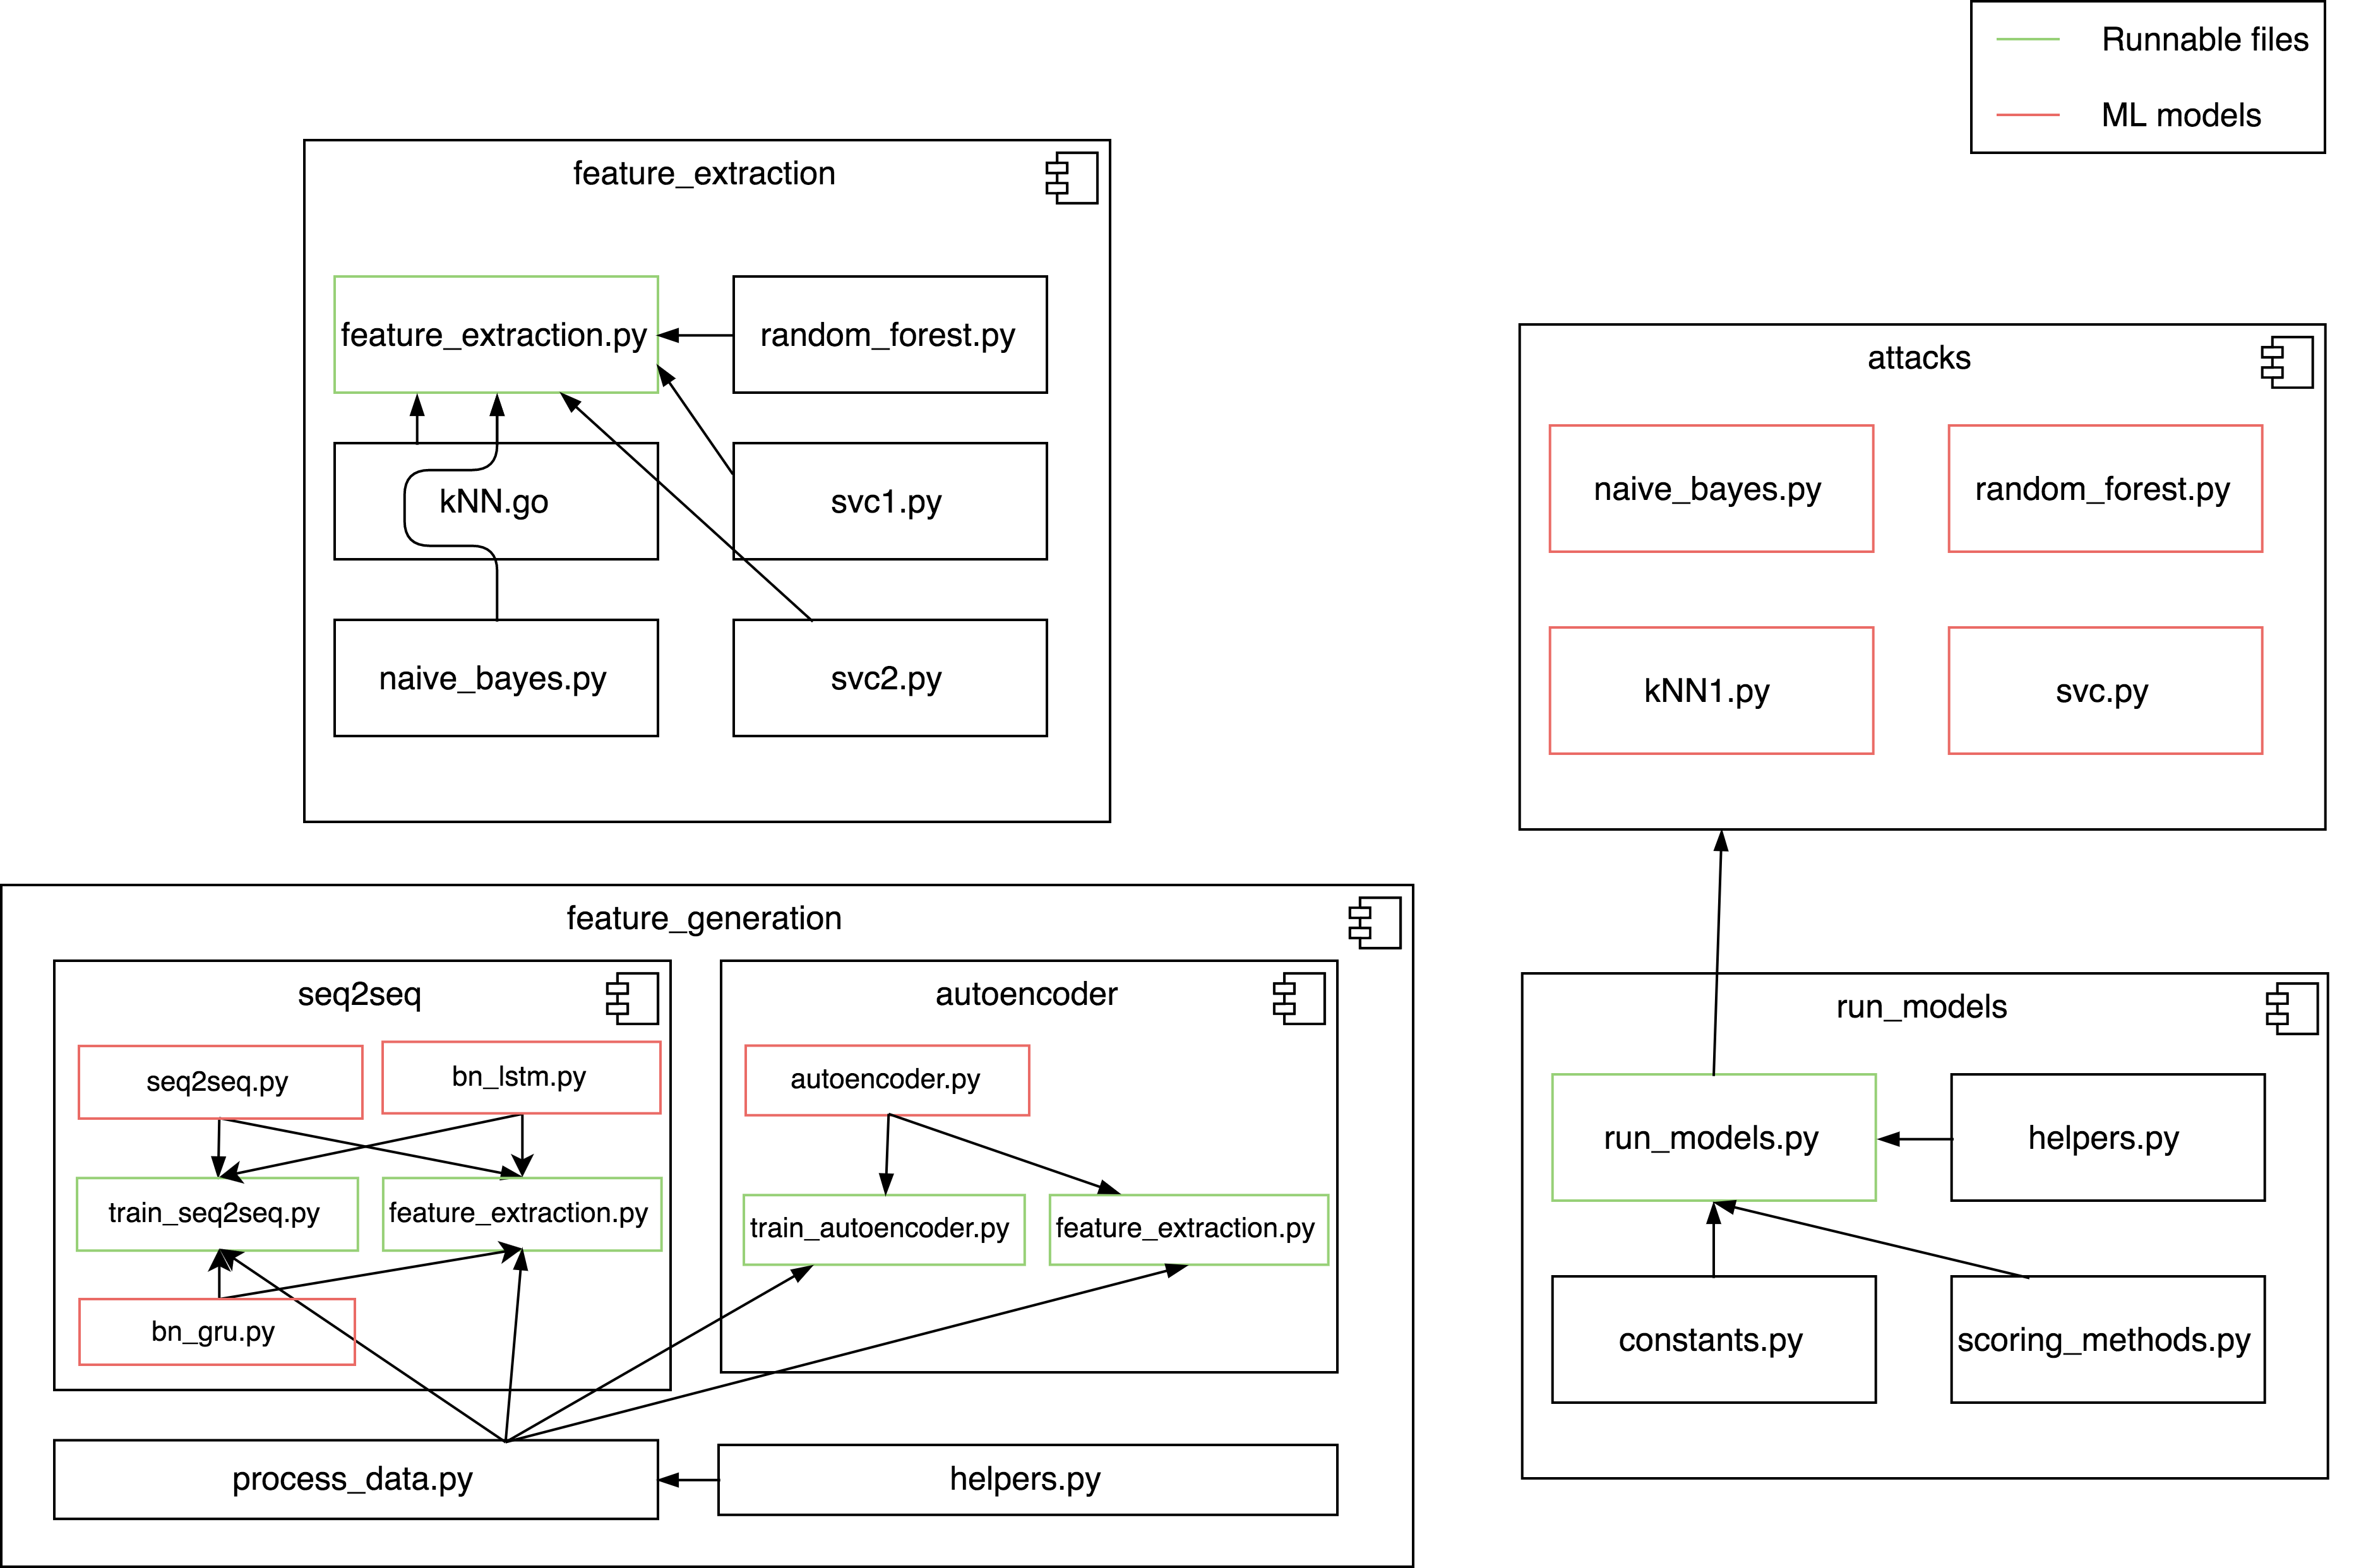
\includegraphics[width=\textwidth]{code-structure}
  \caption{Diagram of how different components are related.}
  \label{fig:code-structure}
\end{figure}

All of the data that is used within this work has already been preprocessed into Tor cells with SENDMEs removed, as described in section \ref{sec:data_collection1}.
The \texttt{feature\_generation} module contains all of the code to further preprocess the data, train the fingerprint extraction models and to extract the fingerprints using the respective model.

The classifiers that will be used for the attacks are defined in the \texttt{attacks} module.
We tried to pick a variety of existing models to measure how well our extracted fingerprints work on different classifiers.
The code to actually test the attacks is defined in the \texttt{run\_models} module, which also does some data preprocessing, defines the logic for the stratified k-fold validation and the different scoring methods.

\newpage

Finally, there is also the \texttt{feature\_extraction} module, which is used to extract hand-picked features from the raw data.

As can be seen, all of the code is written in Python, due to the wide availability of machine learning tools.
Except for the \texttt{kNN.go} file, in the \texttt{feature\_extraction} module, which is adapted from Pylls and written in \textit{Golang} to gain a performance boost \cite{gokNN}.

  \chapter{Evaluation and Testing}

In the following section, we outline how we will be evaluating the suggested model.
Next, we will perform that evaluation and present the final results.

\section{Experimental Setup}

Since our deep model requires a large amount of computation, we like to make use of parallelization.
Hence, all of our experiments that involve the sequence-to-sequence model have been run on an \textit{Amazon EC2 p2.xlarge} instance.
This VM has a \textit{NVIDIA K80 GPU} with 12 GiB of GPU memory.
This instance was then setup with \textit{CUDA 8} and \textit{cuDNN v5.1} \cite{tensorflow,nvidia_developer_2017}.

The rest of the experiments are run on a 2016 MacBook Pro, with a 2.9GHz Intel Core i5 and 8GB of RAM, running MacOS 10.12.
To make sure that the same Python environment is used on both these machines, we consistently use \textit{Python 3.6} and a \textit{virtual environment} for the python dependencies.

As previously mentioned, the main dataset that will be used is \texttt{GRESCHBACH} but we will also be using some of the data in the \texttt{WANG14} dataset to see how the model performs on data that was recorded under different circumstances.
From both these datasets, we will only be using the preprocessed Tor cells and not the raw TCP traffic data.

% TODO: Should I include more here?

\section{Evaluation Techniques}

There are several different manners in how we can evaluate the feature selection process.
First of all, we could analyse the training and test error, as the model learns.
If the training curve suddenly drops, the learning rate might be too high.
Or if the space between both the training and the test error increases, the model will clearly be overfitting.

However, these graphs only show us how well the model is at reproducing the trace from a fingerprint but now how well it performs in a WF attack.
For this we need to train a classifier and see how well it performs by using the metrics described in section \ref{sec:classifier-training}.

To be able to compare these fingerprints with hand-picked ones, we could run the classifier with hand-picked features and with the automatically generated ones.
These hand-picked features are often chosen by experts and after a careful analysis of what the most appropriate features are.
Hence, if the classifier with our fingerprints were to get similar results or even outperform the classifiers with the hand-picked features, we know that the sequence-to-sequence model has been successful.
For these results to be accurate, we do not change any parameters within the classifiers.
Thus everything, except for the features, stays fixed.

For the classifiers, we pick a small set of five existing models.
We aim to pick models that have had an influence on the WF field whilst also having a variety of different classifiers.
This set includes the two \textit{support vector classifiers} (SVCs) used by Panchenko et al. \cite{panchenko1,panchenko2},
the k-fingerprinting attack, which relies on a \textit{random forest} (RF) used by Hayes et al. \cite{kfingerprinting}
and finally the \textit{k-nearest neighbours} (kNN) classifier used by Wang et al. \cite{wang_cai_johnson_nithyanand_goldberg_2014}.

For all of these models, we extract the exact same features as outlined in the respective papers and compare the performance of our generated features compared to the hand-picked ones.
The code for this feature extraction process can be found in the \texttt{feature\_extraction} module.
After analysing all of these features, the most important ones seem to be \cite{panchenko1,panchenko2,kfingerprinting,wang_cai_johnson_nithyanand_goldberg_2014}:

\begin{itemize}
  \item Total number of packets.
  \item Number of incoming packets.
  \item Number of outgoing packets.
  \item Percentage of incoming and outgoing packets.
  \item Concentration of packets.
\end{itemize}

We also aim to use the exact same hyperparameters described in the respective papers. More specifically:
\begin{itemize}
  \item \textbf{SVC} \cite{panchenko1} - a \textit{radial basis function} (RBF) kernel with $C = 2^{17}$ and $\gamma = 2^{-19}$.
  \item \textbf{SVC} \cite{panchenko2} - uses the same hyperparameters as in the previous SVC but with different features.
  \item \textbf{RF} \cite{kfingerprinting} - shows that the best accuracy/time tradeoff is made when $k = 3$ and $\textit{num\_trees} = 20$.
  \item \textbf{kNN} \cite{wang_cai_johnson_nithyanand_goldberg_2014} - also shows that the best accuracy/time tradoff is made when $k = 2$ and $k_{\textit{reco}} = 5$.
\end{itemize}

However, we do need to note that this might have an impact on the performance because these parameters have been specifically tuned for the hand-picked features and not for our fingerprints.

\section{Evaluation}

\subsection{Learning Parameter Tuning}

As mentioned in section \ref{sec:fingerprint-extraction-training}, there are a couple design decisions that need to be made regarding different architectures and learning parameters for the sequence-to-sequence model.
We first try to aim to get the appropriate values for the learning parameters within a simple encoder and decoder with LSTM cells and $120$ hidden states.

First, we start by varying the mini-batch sizes from $20$ to $400$ in steps of $20$.
The higher this value, the longer it takes before making a weight update and the lower the value, the more noise in the training data.
For instance, as can be seen in figure \ref{fig:varying-batch-sizes}, there is clearly a trend of the training error decreases over time.
However, since the batch size is low for the first case, there is a higher probability of having a batch where the training error is high for all of the samples within that batch.
Hence, the data will look very noisy.
Whilst the greater the batch size, the easier to spot this trend.
\begin{figure}[ht]
  \centering
  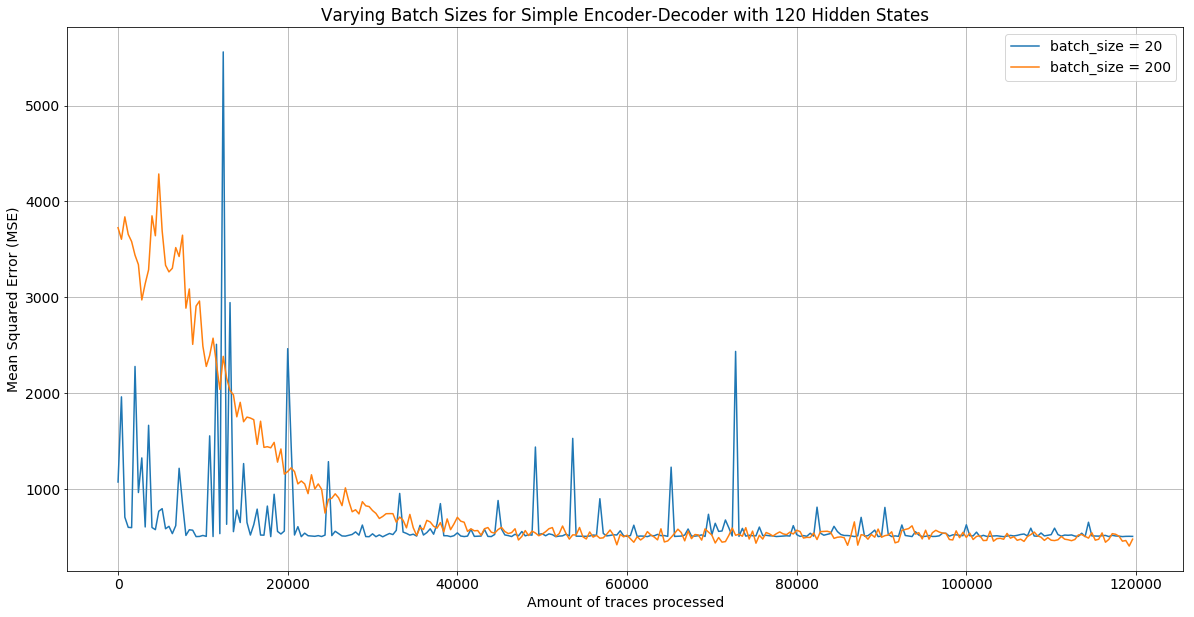
\includegraphics[width=0.9\textwidth]{varying-batch-sizes}
  \caption{Scaled MSE over traces processed for different batch sizes.}
  \label{fig:varying-batch-sizes}
\end{figure}

Preferably we would like to have an even greater batch size than $200$ but due to memory constraints, the model runs out of memory when the amount of hidden states is greater than $100$.
Thus through the rest of the report we will use a mini-batch size of $200$.

Next, we vary the learning rate $\gamma$ from $0.01$ to $0.000001$ with various optimizers (\textit{adam}, \textit{gradient descent} or \textit{RMSProp}) and loss functions (\textit{mean squared error (MSE)} or \textit{absolute loss} (AL)).
As expected, during our experiments, the \textit{adam optimizer} continuously demonstrated better results.

Next, we also noted that the best quality of data compression was achieved with a \textit{MSE loss functio}n and a learning rate of $0.000002$.
Hence, we set $\lambda = 0.000002$, $b = 200$ and use an adam optimizer with MSE for the rest of our experiments.


% TODO: Reversing traces
% TODO: Add cutting traces as a learning parameter

\subsection{Architecture Tuning}

Now that we have an average measure of the learning parameters, we can start changing the architecture of the sequence-to-sequence model to see which ones yield the best results.

% See how it performs on other dataset

\subsection{Classifier Performance}

% Include different models

% Did the design do the job you intended, or were there problems?
% Is your solution fit for purpose?
% How does the resulting system compare against the competition?
% Binary vs multiclass

\section{Unit Tests}

On top of evaluating the results, we also needed to ensure that the results were in fact the the code behaves as we expect it to.
For this we use unit tests.
Some of the code, such as the sequence-to-sequence model is difficult to test but we can still test all of the preprocessing to see if that is correct.
For this we use Python's standard \texttt{unittest} module \cite{python_unittest_documentation}.
The reason for this choice is that it is flexible and the standard unit testing framework, which means it is commonly used.

On top of unit tests, \textit{Travis} was also used \cite{travis}.
Travis is a popular tool, that has an easy integration with Github, for continuous integration.
Therefore, every time a commit is pushed to the remote repository, Travis runs all of the tests automatically.
If one of the tests fails, Travis then automatically notifies all the contributors.

Finally, to check if our tests cover our entire codebase, \textit{codecov} is used \cite{codecov}.
This tool automatically checks how much of the codebase all of the unit tests cover.
At the time of writing, the coverage is $93\%$.
The bits that aren't covered by unit tests, such as the Tensorflow implementation of the sequence-to-sequence model, have been carefully examined to see if they behave as expected.

  \section{Conclusion}

\subsection{Future Works}
- TODO: How it performs against defenses
- TODO: Regularisation
- TODO: Tor hidden services
- TODO: Collecting data over time
- TODO: More realistic user behavior


  \newpage

  % References
  % \clearpage

  \addcontentsline{toc}{section}{Bibliography}

  \nocite{*}
  \printbibliography[title={Bibliography}]

  \newpage

  % Include appendices
  \begin{appendices}
    \titleformat{\section}[display]{\normalfont\Large\bfseries}{\appendixname\enspace\thesection}{.2em}{}
    \chapter{System Manual} \label{appendix:system-manual}

\begingroup

\renewcommand{\thesubsection}{\arabic{subsection}}

\renewcommand{\addcontentsline}[3]{}% Do nothing

Here, we outline the technical details of the project such that the development of the system could be continued by a third party.

First, we will look at the tools required to run the system then we will look at the overall system and how specific modules connect together.
Finally, we explain the specific components and outline how you can contribute to this project.

All of the code is hosted in a private repository on Github.
If given access, it can be cloned from the following url (https://github.com/AxelGoetz/website-fingerprinting.git).

\subsection{Tools Required and Installation Instructions}

Most of the project has been written in Python, more specifically, everything has been designed and tested with version 3.6.
Our Travis build has also been configured to run all of the tests with Python 3.5, which means that we still get notified if anything breaks under a specific Python version.
Some of the code has also been written in Golang, those parts have been adapted from an implementation of Wang et al.'s kNN attack for performance reasons \cite{wang_cai_johnson_nithyanand_goldberg_2014,gokNN}.

Next, after the correct version of Python and Golang are installed, we also require a \textit{virtual environment} to manage all of our python dependencies.
If you have \texttt{pip} on your system, this can easily installed as follows:

\begin{lstlisting}[language=Bash]
pip install virtualenv
\end{lstlisting}

After the virtual environment is installed, go to the project directory and run the following commands to first create the environment and then activate it.

\begin{lstlisting}[language=Bash]
virtualenv venv
source venv/bin/activate
\end{lstlisting}

At any time, you can go out of the virtual environment by running \texttt{deactivate}.
After you are in the environment, we need to install a list of dependencies, which can be found in the \texttt{requirements.txt} file.
This can be done by running:
\begin{lstlisting}[language=Bash]
pip install -r requirements.txt
\end{lstlisting}

This will install a list of dependencies but the main ones are \textit{Tensorflow v1.1}, \textit{numpy}, \textit{sklearn} and \textit{scipy}.
There are a couple others but they are not used for major components.

If you plan to use the GPU support on Tensorflow, there are a couple more steps that need to be taken such as installing \textit{CUDA 8} and \textit{cuDNN v5.1}.
These instructions can be found on the Tensorflow site\footnote{https://www.tensorflow.org/install}.
Our project relied on an Amazon EC2 p2.xlarge with one NVIDIA K80 GPU but the code can be run on any GPU card with CUDA compute capability 3.0 or higher \cite{tensorflow}.

\newpage

In order to run the experiments, the datasets will have to be downloaded next.
The main dataset used is \texttt{GRESCHBACH}\footnote{https://nymity.ch/tor-dns/\#data} but we also use \texttt{WANG14}\footnote{https://cs.uwaterloo.ca/~t55wang/wf.html}.
These should be put in a data folder in the main directory where the directory containing the \texttt{GRESCHBACH} data, should be renamed to \texttt{cells} and the \texttt{WANG14} data to \texttt{WANG14\_cells}.

\subsection{System Overview}

Figure \ref{fig:code-structure} already shows the overall structure of the and how different components interact.
Next, in section \ref{sec:code-structure} we also explain what the individual sections do.
Hence, here we describe the same using a \textit{directory tree}.

\dirtree{%
.1 /.
.2 attacks - Contains the code for all of the classifiers.
.2 data.
.3 cells - All of the individual cell files from the GRESCHBACH dataset.
.2 feature\_extraction - All of the code to extract the hand-picked features from different models.
.2 feature\_generation - Perform automatic feature generation.
.3 autoencoder - Implementation of the autoencoder, how to run it and how to extract features.
.4 autoencoder - Autoencoder class.
.4 feature\_extraction - Used to extract features after model has been trained.
.4 train\_autoencoder - Runnable file for training.
.3 seq2seq - Implementation of the sequence-to-sequence model, how to run it and how to extract features.
.4 seq2seq - Sequence-to-sequence class.
.4 feature\_extraction - Used to extract features after model has been trained.
.4 train\_seq2seq - Runnable file for training.
.2 report - The latex and pdf files for this report.
.2 run\_models - Provides the infrastructure to run a specific attack in the attacks directory.
.2 tests - The unit tests to test everything.
.2 gitignore.
.2 travis.
.2 LICENSE.
.2 README - More information on the project and how to install/run everything.
.2 requirements - The python packages required.
}

\newpage

\subsection{Components}

Here how the individual components work and how to potentially extend them.

\subsubsection{Attacks}

This components implements all of the classifiers that are used to compare the hand-picked features with the automatically generated ones.
Each of these classes needs to implement the interface, which has a \texttt{fit} and \texttt{predict} method.
This is similar to the machine learning models provided in \textit{sklearn} \cite{scikitlearn}.
The fit method takes an $X$ and $y$ input and changes its internal structure such that it minimizes the error.
The predict method on the other hand just takes $X$ as its input and returns a vector $y$ of what it predicts the input represents.

The models should also have a \texttt{is\_multiclass} flag, which represents the fact whether the classifier performs a binary or multiclass classification task.

\subsubsection{Feature Extraction}

All of the logic to extract the hand-picked features for different attacks is in this module.
If a new attack is added, a new file should be created in this directory, with the code to extract all the required features from a given trace.
Next, this function needs to be added to the list in the \texttt{feature\_extraction.py} file.
This file essentially goes over all the traces within the \texttt{data/cells} directory and stores the extracted features within the \texttt{data} directory.

\subsubsection{Feature Generation}

This is one of the main components of this work, containing the code to automatically generate features.
Currently, we have two models defined, namely a sequence-to-sequence model, which can be found in \texttt{seq2seq} and an autoencoder in \texttt{autoencoder}.
In these directories, we first have a file, containing a class that defines a model and then two more files, which are executables, used to train and extract the features (\texttt{train\_<model\_name>.py} and \texttt{feature\_extraction.py}).

When running the training files, after every epoch, the infrastructure will save the computational graph such that training can be continued even if it is interrupted.
The name of these files depend on the Tensorflow version and the model you are training but generally look like \texttt{<model\_name>\_model.meta}.

Finally, all of the logic to actually extract the features is in the \texttt{feature\_extraction.py} files, which again stores the fingerprints in the \texttt{data} directory.

If you wish to implement a new model, add a new directory within the \texttt{feature\_generation} folder with the model name.
Then create three new files, which contain the model definition, training and extracting code.
The model  just needs to implement two main functions such that it can be used by the rest of the infrastructure.
These are \texttt{train\_on\_copy\_task} and \texttt{get\_vector\_representations}, which both take some data as their input and either train the model or extract features.

\newpage

\subsubsection{Run Models}

All of the infrastructure to actually run the classifiers is defined within this module.
First, it defines the logic to preprocess all of the necessary data and perform the \textit{k-fold validation}.
Next, it also defines all of the scoring methods and how to actually run the models.
The main logic is actually in the \texttt{run\_models.py} file, which allows the user to tune certain parameters such that they can run different models.

Whenever a new classifier is added to the \texttt{attacks} directory, it should also be added within the \texttt{run\_models.py} file such that a user knows that it can be run.

\subsubsection{Unit Tests}

For unit testing, we use the standard \texttt{unittest} module, which is very simple to use.
To create more tests, create a new file in the \texttt{tests} directory, which starts with test and then the name of what you will be testing.
Next, create a class within that file, which extends the \texttt{unittest.TestCase} class and add the methods of what you would like to test.

Then to run all of the unit tests within the \texttt{tests} directory, simply run:
\begin{lstlisting}[language=Bash]
python -m unittest discover
\end{lstlisting}

\subsection{Contributing}

There are a variety of different extensions possible, some of which are outlined in section \ref{sec:future-works}.
If you decide to implement one of these, we use a very standard git workflow so if you would like to contribute, follow these steps:

\begin{enumerate}
  \item Fork the project repo.
  \item Create a branch with the name of the particular improvement/extension that you will be working on.
  \item After you are done, make sure that you run all of the tests and check if everything still works.
  \item Submit a pull request from your branch to the master branch and make sure all of the tests pass on Travis.
\end{enumerate}

If you discover an issue or want to work on an extension, please create an issue on our Github issues page to let people know that you are working on this particular extension.

\subsubsection{Style Guide}

When contributing, please do note that we try to adhere to the \textit{PEP 8}\footnote{https://www.python.org/dev/peps/pep-0008/} style guide for our python code \cite{pythonpep8}.
This is done for consistency reasons and readability of the code.

Although it is not necessary to adhere to all of the guidelines, we strongly suggest for you to adhere to the basics.
If the code within a pull request is unreadable or does not adhere to any of the standards, there is a very strong change that it will not be merged.

\endgroup

    \chapter{User Manual}

    \newpage
\chapter{Project Plan}

\setcounter{secnumdepth}{5}
\begingroup

\renewcommand{\thesubsection}{\arabic{subsection}}

\renewcommand{\addcontentsline}[3]{}% Do nothing

\subsection{Problem Statement}
Anonymity networks like Tor use what is called onion routing where each layer in the onion represent a new layer of encryption.
This allows Tor users to freely browse the web without an ISP, government, or anyone else that might be able to sniff the traffic before the first Tor node to see which websites or services the user is accessing.
However even with various layers of encryption, an attacker might still be able to infer which web page a client is browsing by performing a \textit{website fingerprinting attack}.
The attack often uses machine learning to identify several trends in the network traffic such as the number of packets per second, their size, etc.
But most of these attacks rely on a trail and error process of picking the features.
Hence, there is no guarantee that the features used are the most appropriate ones or even any good at all.
Therefore this project will analyse the use deep learning techniques such as stacked autoencoders to automatically identify features and test their effectiveness compared to the hand-picked ones in various different models.

\subsection{Aims and Objectives}
The aims and objectives for this project are as follows:
  \begin{enumerate}
    \item \label{aim1} \textbf{Aim:} Critically review the effectiveness of current website fingerprinting attacks.\\
    \textbf{Objectives:}
    1. Analyse various models that are currently used in fingerprinting attacks.
    2. See if there are any flaws in the reasoning or the experimentation.
    3. Examine how would a small percentage of false positives impacts a potential attack.
    4. Analyse how the rapid changing nature of some web pages would impact the attack.

    \item \textbf{Aim:} Generate features automatically using deep learning techniques for a website fingerprinting attack.\\
    \textbf{Objectives:}
    1. Examine different deep learning feature selection methods such as stack autoencoders.
    2. Pick the most appropriate method for a website fingerprinting attack.
    3. Collect the necessary data to train the feature selection method. This includes a dataset that is collected over a short period of time (days) and another one that would be collected over an extended period of time (weeks).
    4. Extract a set of features using this data.
    5. Compare these features to existing hand-picked ones.
\newpage
    \item \textbf{Aim:} Train existing models with the automatically generated features and test their effectiveness compared to hand-picked ones.\\
    \textbf{Objectives:}
    1. Identify various models that could be used to test the new features with.
    2. Implement the models.
    3. Identify various sets of hand-picked features to compare the automatically generated features with.
    4. Train those models using both hand-crafted features and the generated features.
    5. Compare the effectiveness of the generated features to hand-picked ones in those models in a closed-world environment.
    6. Compare their effectiveness in an open-world scenario.
    7. Analyse if the feature selection technique can find persistent features that are spread across a period of time and study if this helps with the classification over time.
    8. Compare the effectiness of the automatically generated features when a user uses various common defeneses against website fingerprinting like camouflage.
    9. Test the attack on tor hidden services as opposed to websites.
    10. Investigate an appropriate technique for evaluating the result.
    11. Analyse which features tend to be the most informative (highest entropy).

  \end{enumerate}

\subsection{Deliverables}
The project aims to produce the following deliverables:
\begin{enumerate}
  \item Summary of website fingerprinting attacks. This includes any related work and an analysis how effective a fingerprinting attack could be (see Aim \ref{aim1}).
  \item An analysis of the most appropriate automatic feature generation model.
  \item A dataset to train both the feature generation model and the models used for the website fingerprinting attack.
  \item Fully documented source code for generating the features and the models used for the attack.
  \item A strategy for testing the models.
  \item An analysis of using the generated features compared to hand-picked one using diferent models. This includes how the feature generation process might be able to identify persistent features that are spread across a period of time.

\end{enumerate}

\newpage

\subsection{Work Plan}
  \textbf{Project start to end October (4 Weeks)}\\
  \indent Research current website fingerprinting attacks.\\
  \indent Research various method for automatic feature selection.\\
  \\
  \textbf{Mid-October to mid-November (4 Weeks)}\\
  \indent Refine aims and objectives.\\
  \indent Further research into using automatic feature selection for website fingerprinting attacks.\\
  \\
  \textbf{November (4 weeks)}\\
  \indent Collect necessary data.\\
  \indent Initial experimentation with feature selection.\\
  \\
  \textbf{End November to mid-January (8 weeks)}\\
  \indent Implement feature selection.\\
  \indent Implementation of various models used for attacks.\\
  \indent Research on how to evaluate the effectiveness of a model.\\
  \indent Work on the Interim Report.\\
  \\
  \textbf{Mid-January to mid-February (4 weeks)}\\
  \indent Perform tests and evaluate the performance.\\
  \\
  \textbf{Mid-February to end of March (6 weeks)}\\
  \indent Work on Final Report.\\
  \\

\endgroup

    \chapter{Interim Report}

\begingroup

\renewcommand{\thesubsection}{\arabic{subsection}}

\renewcommand{\addcontentsline}[3]{}% Do nothing

\subsection{Current Progress}
We have updated some requirements that were mentioned in the project plan.
Rather than first collecting a large dataset of website traces over a long period of time,
we decided to start with existing datasets to perform some experiments. Then later, if we get the opportunity to do so, we can still collect our own data.

Given the nature of the challenge, a majority of the time will be spend on researching models that perform automatic feature selection.
After careful examination, there are only two couple deep learning methods that seem to be appropriate, a \textit{RNN Encoder Decoder} or a \textit{Bidirectional RNN Encoder}.
We also considered using a \textit{Stacked Autoencoder}  but it did not seem to be appropriate as it requires a fixed-length vector as an input.
Hence, if we were to use it, we either have to pad or compress the traces, which are both not elegant solutions.
In addition to simply training these models on the data, we might perform \textit{denoising} on the them, which essentially means learning the models to distinguish uncorrupted data from corrupted data.
This final step allows us to fine tune the encoders to get a consistent performance even if some of the data is noisy.

Although we have started experimenting with some of these models, they have not been fully implemented.
However we are still on schedule for doing so.

Finally, we have also selected a set of previously successful website fingerprinting attacks.
An environment has been set up, some of these models have been implemented and the infrastructure is in place to extract a set of hand-picked features from the raw data.
This will allow us to quickly perform a performance comparison with the manually engineered features and the automatically selected ones.

\subsection{Remaining Work}
The first priority is to fully implement a \textit{RNN Encoder Decoder} or a \textit{Bidirectional RNN Encoder} and fine tune it.
Next, we have to perform the analysis on how appropriate our automatically engineered features are compared to hand-picked ones.
So this includes finishing the implementation of existing models, and the infrastructure to extract the features.

Next, we need to pick a set of criteria that we will use to compare the predictive power of several models.
Using these criteria we will then have to perform a thorough analysis of how the automatically engineered features compared to the hand-picked ones.

Finally, after all of the above has been completed, we will focus on finished writing the final report.
If there is still time remaining, we might still try to collect our own data over an extended period of time

\endgroup

  \end{appendices}

\end{document}
